\newcommand{\DeinName}{Pascal Fischer}
\newcommand{\MatrNo}{371778}
\newcommand{\TitelArbeit}{Entwicklung einer verschlüsselten Chat-basierten Plattform auf Basis des Matrix.org-Protokolls im Kontext von digitaler Gesundheit und Telemedizin}
\newcommand{\Fachgebiet}{Regelungssysteme}
\newcommand{\PrueferEins}{Dr.-Ing Thomas Schauer}
\newcommand{\PrueferZwei}{Prof.-Dr.-Ing. Clemens Gühmann}
\newcommand{\fachbereich}{Elektrotechnik und Informatik}

% entweder ein Datum h?ndisch eintragen, oder den Befehl \today nutzen
\newcommand{\Datum}{\today}

\makeglossary


%
% Einbinden des Headers, hier k?nnen auch weitere Einstellungen vorgenommen werden.
%%%%%%%%%%%%%%%%%%%%%%%%%%%%%%%%%%%%%%%%%%%%%%%%%%%%%%%
%																					%
%	In dieser Datei werden alle Packages eingebunden, 	%
% welche f�r das Dokument n�tig sind. Desweiteren 		%
% werden die Dokumentinformationen gesetzt.						%
%																											%
%%%%%%%%%%%%%%%%%%%%%%%%%%%%%%%%%%%%%%%%%%%%%%%%%%%%%%%
%
%	Die KOMAScript Dokumentklasse "scrbook" verwenden.
%
\documentclass[pdftex, 		%
							a4paper, 		% DIN A4 verwenden
							titlepage,	% separate Titelseite
							%draft,			%	Draft-Version, keine Bilder im pdf!
							final,			% Final-Version
							oneside,		% einseitiger Druck
							12pt,				% Schriftgr��e 12pt
							DIV=calc,
							%tocbasic,
							]{scrbook}	%	KOMAScript scrbook-Dokumentklasse

							\usepackage{geometry}
							\geometry{
								left=3cm,
								right=3cm,
								top=3cm,
								bottom=4cm,
								bindingoffset=5mm
							}

\usepackage{tikz}

%%%%%%%%%%%%%%%%%%%%%%%%%%%%%%%%%%%%%%%%%%%%%%%%%%%%%%%%
%	Einbinden der Pakete
%%%%%%%%%%%%%%%%%%%%%%%%%%%%%%%%%%%%%%%%%%%%%%%%%%%%%%%%

\usepackage[ngerman]{babel}

% PDF Dateien einbinden
\usepackage{pdfpages}

%Settings for PDF Pages to accept additonal versioned PDF files
\pdfminorversion=6
\pdfcompresslevel=9
\pdfobjcompresslevel=9

%Infos dazu unter: http://www.bakoma-tex.com/doc/latex/koma-script/scrhack.pdf
%Einige Pakete haben Probleme mit dem Komaskript.
\usepackage{scrhack}


% Definieren von eigenen benannten Farben.
% F�r sp�tere Verwendung in dem Dokument, definieren wir einzelne
% benannte Farben.
%
\usepackage{xcolor}
\definecolor{gray1}{gray}{0.92}
\definecolor{darkgreen}{rgb}{0,0.5,0}

\definecolor{urlLinkColor}{rgb}{0,0,0.5}
\definecolor{LinkColor}{rgb}{0,0,0}
\definecolor{ListingBackground}{rgb}{0.85,0.85,0.85}

\usepackage{pgf-umlsd}

\definecolor{delim}{RGB}{20,105,176}
\definecolor{numb}{RGB}{106, 109, 32}
\definecolor{string}{rgb}{0.64,0.08,0.08}
\rmfamily
\usepackage{amsfonts}
\usepackage[square,numbers]{natbib}
\usepackage{palatino}
\usepackage{amsmath}				% Schriftfamilie Palatino
%\usepackage[utf8]{inputenc}
%\usepackage[latin1]{inputenc} % Umlaute
\usepackage[utf8]{inputenc}
%\usepackage[dvips]{color}    	% f�r graue Boxen
%\usepackage[dvips]{graphicx} 	% Grafikpaket
\usepackage{multirow}
\usepackage{graphicx}
%\usepackage[table,xcdraw]{xcolor}
\usepackage{makeidx}   				% Paket zur Erzeugung eines Index
\usepackage{siunitx}
\sisetup{locale = DE}
\usepackage[normalem]{ulem}   % bietet Unterstreichungsvarianten
%\usepackage{picins} 					% Bilder im Absatz platzieren
\usepackage[T1]{fontenc}			% Erweiterten Zeichensatz aktivieren
\usepackage{multido}					% erm�glicht Schleifenartiges wiederholen von Befehlen
\usepackage{mdwlist}					% erm�glicht das Setzen des Z�hlers bei Aufz�hlungspunkten
\usepackage{paralist}					% Paket f�r Aufz�hlungen, erweitert Enumerate-Paket
\usepackage{longtable}				% mehrseitige Tabellen
\usepackage{tocbasic}
\parindent0pt           			% verzichte auf Einr�cken der ersten Zeile
\parskip1ex             			% Abstand zwischen den Abs�tzen

\usepackage{setspace}					% Paket zum Einstellen des Zeilenabstands
\onehalfspacing								% anderthalbfacher Zeilenabstand
%\doublespacing								% doppelter Zeilenabstand
%\singlespacing								% einfacher Zeilenabstand
\usepackage{float}
%\usepackage[german]{babel}
\usepackage[german=quotes]{csquotes} %Deutsche Anf�hrungszeichen
\usepackage{subfig}
\definecolor{LinkColor}{rgb}{0.1,0.1,0.1}
%\definecolor{ListingBackground}{rgb}{0.85,0.85,0.85}
\definecolor{ListingBackground}{rgb}{0.98,0.98,0.98}
\definecolor{gray}{rgb}{0.4,0.4,0.4}
\definecolor{darkblue}{rgb}{0.0,0.0,0.6}
\definecolor{cyan}{rgb}{0.0,0.6,0.6}



%
% Farbeinstellungen f�r die Links im PDF Dokument.
%
\makeindex

%-----------Paket f�r absolute Positionierung von Grafiken------------------
\usepackage[absolute]{textpos}
\setlength{\TPHorizModule}{1mm}
\setlength{\TPVertModule}{\TPHorizModule}

%-----------Aufz�hlungen und Einstellungen f�r Sourcecode-------------------
%\usepackage[savemem]{listings} %Bei wenig Arbeitsspeicher dies Option [savemem] aktivieren.
\usepackage{listings}
\lstloadlanguages{TeX,XML, Java} % TeX sprache laden, notwendig wegen option 'savemem'
\lstset{%
	language=[LaTeX]TeX,     % Sprache des Quellcodes ist TeX
	numbers=left,            % Zelennummern links
	stepnumber=1,            % Jede Zeile nummerieren.
	numbersep=5pt,           % 5pt Abstand zum Quellcode
	numberstyle=\tiny,       % Zeichengr�sse 'tiny' f�r die Nummern.
	breaklines=true,         % Zeilen umbrechen wenn notwendig.
	breakautoindent=true,    % Nach dem Zeilenumbruch Zeile einr�cken.
	postbreak=\space,        % Bei Leerzeichen umbrechen.
	tabsize=2,               % Tabulatorgr�sse 2
	basicstyle=\ttfamily\footnotesize, % Nichtproportionale Schrift, klein f�r den Quellcode
	showspaces=false,        % Leerzeichen nicht anzeigen.
	showstringspaces=false,  % Leerzeichen auch in Strings ('') nicht anzeigen.
	extendedchars=true,      % Alle Zeichen vom Latin1 Zeichensatz anzeigen.
	backgroundcolor=\color{ListingBackground}} % Hintergrundfarbe des Quellcodes setzen.


\lstset{
  basicstyle=\small\ttfamily,
  columns=fullflexible,
  showstringspaces=false,
  %commentstyle=\color{gray}\upshape
}
%neue Lang definieren, als Bsp.
\lstdefinelanguage{XML-changed}
{
  basicstyle=\footnotesize\ttfamily\bfseries,
  morestring=[b]",
  morestring=[s]{>}{<},
  morecomment=[s]{<?}{?>},
  stringstyle=\color{black},
  identifierstyle=\color{darkblue},
  keywordstyle=\color{cyan},
  morekeywords={xmlns,version,type}% list your attributes here
}

%-----------Caption Package-------------------
\usepackage{caption}
\DeclareCaptionFont{white}{\color{white}}
\DeclareCaptionFormat{listing}{\colorbox[cmyk]{0.43, 0.35, 0.35,0.01}{\parbox{\textwidth}{\hspace{15pt}#1#2#3}}}

\DeclareCaptionFormat{graphics}{\colorbox[cmyk]{0.43, 0.35, 0.35,0.01}{\parbox{\textwidth}{\hspace{15pt}#1#2#3}}}


\captionsetup[lstlisting]{format=listing,labelfont=white,textfont=white, singlelinecheck=false, margin=0pt, font={footnotesize}}

%-----------Header+Footer---------------------------------------------------
\usepackage{fancyhdr}					%
\pagestyle{fancy}							%

\fancyhead{}
\fancyfoot{}
\renewcommand{\headrulewidth}{0.4pt} % Kopzeilenlinie
\renewcommand{\footrulewidth}{0.0pt} % Fusszeilenlinie 0.0pt blendet sie aus

\renewcommand{\chaptermark}[1]{\markboth{\thechapter\quad#1}{}}
\renewcommand{\sectionmark}[1]{\markright{\thesection\quad#1}}

%\fancyhead[LO]{\small\sffamily\rightmark}
\fancyhead[LE,RO]{\slshape \rightmark}
\fancyhead[LO,RE]{\slshape \leftmark}
%\fancyhead[RO]{\small\sffamily\thepage}
\fancyfoot[C]{\thepage}

%-----------Um die Eidesstattliche Erkl�rung als PDF einzubinden-----------------------------------
%\usepackage{pdfpages}

%------------Glossar--------------------------------------------------------------
\usepackage{expdlist}
\usepackage{/home/pfischer/Uni/Bachelorarbeit/Bachelorarbeit/paper/src/glossar}

\renewcommand{\glshead}{\chapter*{Glossar}}
\renewcommand{\glentry}[2]{\glossary{#1@[#1] #2|glspage}}
\renewcommand{\glsgroup}[1]{{\listpart{\makebox[0pt][l]{\rule[-2pt]{\textwidth}{0.5pt}}{\textbf{\large #1}}}}}

\makeglossary

%Glossar mit Bordmitteln ------------------------------------------------------------------
%Darstellung des Glossars einstellen
%\usepackage[style=super, header=none, border=none, number=none, cols=2, toc=true]{glossary}
%\renewcommand{\glossaryname}{Glossar}
%\printglossary

% --- diverse Schriften -------------------------------------------------------------------
%\newcommand{\url}[1]{{\sf\small #1}}     % Hyperlinks


% -------F�r ToDo-Notes--------------------------------------------------------------------
\usepackage[color=red, shadow]{todonotes} % ", disable" deaktiviert ToDo-Notes
%Vereinfachtes "Inline-Todo"
\newcommand{\td}[1]{{\todo[inline]{#1}}}
\newcommand{\tdu}[1]{{\todo[inline, color=green!40]{#1}}}

\newcommand{\SubItem}[1]{
	{\setlength\itemindent{15pt} \item[-] #1}
}
\newcommand{\citepnum}[1]{[\citenum{#1}]}

%--------F�r Links-------------------------------------------------------------------------




%--------HyperRef konfigurieren-------------------------------------------------------------------------

\usepackage[
	pdftitle={\TitelArbeit},
	pdfauthor={\DeinName},
	pdfsubject={\TitelArbeit},
	pdfcreator={MiKTeX, LaTeX with hyperref and KOMA-Script auf Basis der Vorlage von seiler.it},
	pdfkeywords={Abschlussarbeit, TU Berlin, Universität},%weitere Keywords hier einf�gen
	pdfpagemode=UseOutlines,%
	pdfdisplaydoctitle=true,%
	pdflang=de%
]{hyperref}

\hypersetup{%
	colorlinks=true,%        Aktivieren von farbigen Links im Dokument (keine Rahmen)
	linkcolor=LinkColor,%    Farbe festlegen.
	citecolor=LinkColor,%    Farbe festlegen.
	filecolor=LinkColor,%    Farbe festlegen.
	menucolor=LinkColor,%    Farbe festlegen.
	urlcolor=LinkColor,%     Farbe von URL's im Dokument.
	bookmarksnumbered=true%  �berschriftsnummerierung im PDF Inhalt anzeigen.
}

\newcommand{\improvement}{\todo[inline, color=green]}
\newcommand{\change}{\todo[inline, color=blue]}
\newcommand{\unsure}{\todo[inline, color=violet]}
\newcommand{\eunorm}[1]{\lVert #1 \rVert_{\num{2}}}
\newcommand{\anfzch}[1]{\glqq #1\grqq{}}


\usepackage{enumitem}

\usepackage{tabularray}
% --------- Generates Chapter header ------------------------

\DeclareMathAlphabet\EuRoman{U}{eur}{m}{n}
\SetMathAlphabet\EuRoman{bold}{U}{eur}{b}{n}
\newcommand{\eurom}{\EuRoman}
\definecolor{nicered}{rgb}{.647,.129,.149}
\usepackage{etoolbox}

\makeatletter
\newsavebox{\feline@chapter}
\newcommand\feline@chapter@marker[1][4cm]{%
	\sbox\feline@chapter{%
		\resizebox{!}{#1}{\setlength{\fboxsep}{0pt}%
		\colorbox{white}{\color{black}$\eurom\thechapter$}}}%
	\raisebox{\depth}{\usebox{\feline@chapter}}%
}
\renewcommand*{\chapterformat}{%
	\sbox\feline@chapter{\feline@chapter@marker[1.61cm]}%
	\makebox[0pt][l]{%
		\makebox[\dimexpr\textwidth][r]{%
			\usebox\feline@chapter}}%
}
\makeatother

\preto\chapterheadendvskip{%
	\vspace*{-\parskip}%
	{\noindent\setlength\parfillskip{0pt plus 1fil}\rule{\textwidth}{.4pt}\par}%
}


\graphicspath{ {./source/images/pictures/} }

\lstdefinelanguage{json}{
    numbers=left,
    numberstyle=\small,
    frame=single,
    rulecolor=\color{black},
    showspaces=false,
    showtabs=false,
    breaklines=true,
    postbreak=\raisebox{0ex}[0ex][0ex]{\ensuremath{\color{gray}\hookrightarrow\space}},
    breakatwhitespace=true,
    basicstyle=\ttfamily\small,
    upquote=true,
    morestring=[b]",
    stringstyle=\color{string},
    literate=
    *{0}{{{\color{numb}0}}}{1}
        {1}{{{\color{numb}1}}}{1}
        {2}{{{\color{numb}2}}}{1}
        {3}{{{\color{numb}3}}}{1}
        {4}{{{\color{numb}4}}}{1}
        {5}{{{\color{numb}5}}}{1}
        {6}{{{\color{numb}6}}}{1}
        {7}{{{\color{numb}7}}}{1}
        {8}{{{\color{numb}8}}}{1}
        {9}{{{\color{numb}9}}}{1}
        {\{}{{{\color{delim}{\{}}}}{1}
        {\}}{{{\color{delim}{\}}}}}{1}
        {[}{{{\color{delim}{[}}}}{1}
        {]}{{{\color{delim}{]}}}}{1},
}


\newcommand\YAMLcolonstyle{\color{red}\mdseries}
\newcommand\YAMLkeystyle{\color{black}\bfseries}
\newcommand\YAMLvaluestyle{\color{blue}\mdseries}

\makeatletter

% here is a macro expanding to the name of the language
% (handy if you decide to change it further down the road)
\newcommand\language@yaml{yaml}

\expandafter\expandafter\expandafter\lstdefinelanguage
\expandafter{\language@yaml}
{
    keywords={true,false,null,y,n},
    keywordstyle=\color{darkgray}\bfseries,
    basicstyle=\YAMLkeystyle,                                 % assuming a key comes first
    sensitive=false,
    comment=[l]{\#},
    morecomment=[s]{/*}{*/},
    commentstyle=\color{purple}\ttfamily,
    stringstyle=\YAMLvaluestyle\ttfamily,
    moredelim=[l][\color{orange}]{\&},
    moredelim=[l][\color{magenta}]{*},
    moredelim=**[il][\YAMLcolonstyle{:}\YAMLvaluestyle]{:},   % switch to value style at :
    morestring=[b]',
    morestring=[b]",
    literate =    {---}{{\ProcessThreeDashes}}3
        {>}{{\textcolor{red}\textgreater}}1
        {|}{{\textcolor{red}\textbar}}1
        {\ -\ }{{\mdseries\ -\ }}3,
}

% switch to key style at EOL
\lst@AddToHook{EveryLine}{\ifx\lst@language\language@yaml\YAMLkeystyle\fi}
\makeatother

\newcommand\ProcessThreeDashes{\llap{\color{cyan}\mdseries-{-}-}}


% Beginn des Dokuments
\begin{document}

%Zitiert alle Referenzen, ohne Sie hier zu listen. Dadurch erscheinen alle Quellen im %Literaturverzeichnis, auch wenn sie im Text nicht genutzt werden.
%Bitte nur f?r Testzwecke verwenden.
    \nocite{*}


% Einbinden des Deckblatts

    \frontmatter
    % erste Seite (Titelseite) der Diplomarbeit mit Titel, Name usw...

\newsavebox{\Prof}
\savebox{\Prof}{Erster Prüfer }

\newsavebox{\Betr}
\savebox{\Betr}{Zweiter Prüfer }
\begin{titlepage}

%\begin{minipage}[h]{0.5\textwidth}
%		\raggedright
%		\includegraphics[height=4cm]{source/images/Logo/TU-Berlin-Logo.png}
%	\end{minipage}
%	\begin{minipage}[h]{0.5\textwidth}
%		\raggedleft
%		\includegraphics[height=5cm]{source/images/Logo/sensorstim_logo.png}
%	\end{minipage}


	\begin{figure}
		\begin{center}
			
\includegraphics[height=4cm]{source/images/Logo/TU_Berlin_Logo.png}
		\end{center}
	\end{figure}

	\begin{center}
%\includegraphics[height=2cm]{source/images/logo_mirolab.png}

	{\Large Technische Universität Berlin}\\[1mm]
	{\large Fakultät Elektrotechnik und Informatik}\\
	{\large Fachgebiet \Fachgebiet}\\
	\vspace{1cm}
	{\LARGE  Bachelorarbeit}

	\vspace{0.5cm}

	{\LARGE\textbf{ \TitelArbeit}}\\


	\vspace{1.cm}

	von\\[2mm]

	\textbf{\large{\DeinName}}\\
%\vspace{1.5cm}
	Matrikelnummer: \MatrNo\\[1cm]

	Betreuer: Ardit Dvorani\\[2mm]

	\usebox{\Prof: \PrueferEins} \\
	\usebox{\Betr: \PrueferZwei} \\

	\vspace{1cm}
	Berlin, \today
	\end{center}
\end{titlepage}
    \hypersetup{pageanchor=false}

    \newpage
    \section*{Zusammenfassung}
    In dieser Arbeit befasse ich mich mit ....

    \section*{Abstract}\label{sec:abstract}
    This paper describes how to ...
    \newpage
    \chapter*{Eidesstattliche Erklärung}\label{ch:eidesstattliche-erklarung}
    Hiermit erkläre ich, dass ich die vorliegende Arbeit selbstständig und eigenhändig sowie ohne
    unerlaubte fremde Hilfe und ausschließlich unter Verwendung der aufgeführten Quellen und
    Hilfsmittel angefertigt habe.\\
    \vspace{1cm}\\
    Berlin, den \underline{\hspace{3cm}} \hfill \DeinName \underline{\hspace{4cm}}

    \newpage
    \tableofcontents

    \mainmatter

    \newpage
    \chapter{Einleitung}\label{ch:einleitung}

    \section{Motivation}\label{sec:motivation}
    Die Digitalisierung findet immer Einzug in unser alltägliches Leben, so auch in der Medizin.
    Besonders seit Beginn der Coronapandemie im Jahr 2019 werden Rufe nach Softwarelösungen für den Einsatz in der Telemedizin immer lauter.
    Da viele gängige Messenger wie Whatsapp oder Telegramm nicht den Datenschutz Vorschriften der DSGVO entsprechen müssen hierfür Alternativen geschaffen werden.


    \newpage
    \section{Zielsetzung}\label{sec:zielsetzung}
    Ziel dieser Arbeit ist es eine Plattform zu entwickeln welchen es Ärzten und Patienten ermöglicht in Kontakt zu treten und Nachrichten auszutauschen.
    Hierfür soll eine Chat-App auf basis des Matrix.org-Protokolls implementiert werden.
    Die App ist in der Programmiersprache Swift zu entwickeln und soll auf allen gängigen iOS Geräten unterstützt werden.
    Darüber hinaus muss die benötigte Infrastruktur bereitgestellt werden um Nachrichten und Daten zu speichern und zu übermitteln.
    Diese soll jedoch isoliert laufen und nicht an das existierende Matrix Netzwerk angeschlossen werden.
    Da medizinische Daten dem Datenschutz in besonderer Maße unterliegen ist es besonders wichtig,
    dass jegliche Art von Kommunikation zwischen Ärzten und Patienten stets verschlüsselt ist.
    Es muss gewährleistet sein, dass zu jedem Zeitpunkt alle personenbezogenen Daten vor dem Zugriff unerlaubter Dritter geschützt sind.
%    Da es im Bereich der Medizin  hinaus ist zu beachten, dass das Userinterface
%    So sollte beispielsweise darauf geachtet werden, dass Da es im Bereich der Medizin hinaus ist zu beachten, dass das Userinterface
%    So sollte beispielsweise darauf geachtet werden, dass

    \section{Aufbau der Arbeit}\label{sec:aufbau-der-arbeit}
    Zuerst werden die Theoretischen Grundlagen
%    Zuerst werden die gesetzlichen Ansprüche an eine Messaging-Plattform im medizinischen Bereich beleuchtet.
%    Anschließend wird das Matrix Protokoll vorgestellt und seine allgemeine Funktionsweise beschrieben.
%    Außerdem werden die zur Verschlüsselung verwendeten Algorithmen erklärt und die dafür benötigten Schlüssel aufgezeigt.
    Es werden die zur Implementierung der Plattform genutzten Technologien vorgestellt und deren Verwendung beschrieben.
    Danach werden einige ähnlicher Projekte vorgestellt und analysiert.
    Basierend auf dieser Analyse werden eine eine Reihe von technischen Anforderungen definiert welche von der implementierten Plattform erfüllt werden sollen.
    Anschließend wird die implementierte Plattform vorgestellt und deren Funktionsweise erklärt.
    Abschließend wird Plattform unter betrachtung der definierten Anforderungen evaluiert.

    \newpage
    \chapter{Theoretische Grundlagen}\label{ch:theoretische-grundlagen}
    In diesem Kapitel werden zunächst die theoretischen Grundlagen, welche die Implementierung der Plattform beeinflusst haben, vermittelt.
    Zuerst werden die gesetzlichen Ansprüche an eine Messaging-Plattform im medizinischen Bereich beleuchtet.
    Anschließend wird das Matrix Protokoll vorgestellt und seine allgemeine Funktionsweise beschrieben.
    Außerdem werden die zur Verschlüsselung verwendeten Algorithmen erklärt und die dafür benötigten Schlüssel aufgezeigt.
    Es wird das REST Paradigma vorgestellt, welches die Grundlage für die Kommunikation zwischen Client und Server bildet.
    Des weiteren wird die MVVM Architektur erläutern, welche bei der Entwicklung der App verfolgt wurde.

    \section{Datenschutz im Gesundheitswesen}\label{sec:datenschutz-im-gesundheitswesen}
    Die Rechtlichen Rahmenbedingungen für das Speicher und Verarbeiten medizinischer Daten sind in der EU-Datenschutz-Grundverordnung\footnote{https://dsgvo-gesetz.de/} (DSGVO) festgelegt.
    Diese fordert ebenfalls zur Einhaltung des IT-Sicherheitsgesetzes und des E-Health-Gesetzes auf.
    Medizinische Daten werden vom Gesetzgeber im besonderem Maße geschützt, da sie besonders sensible Informationen enthalten~\cite{datenschutzimgesundeitswesen}.

    \textit{Das am 29. Dezember 2015 in Kraft getretene "Gesetz für sichere digitale Kommunikation und Anwendungen im Gesundheitswesen (E-Health-Gesetz)" hat die ersten Weichen für den Aufbau der sicheren Telematikinfrastruktur (TI) und die Einführung medizinischer digitaler Anwendungen gestellt.
    Ziel dieses Gesetzes war es, die Chancen der Digitalisierung für die Gesundheitsversorgung zu nutzen und eine schnelle Einführung medizinischer Anwendungen für die Patientinnen und Patienten zu ermöglichen.}~\cite{ehealthgesetz}

    Ein Teil der Telematikinfrastruktur ist der TI-Messenger der Gematik GmbH welcher im Abschnitt~\ref{subsec:ti-messenger} genauer betrachtet wird.\\
    Am 07.11.2019 hat dann die Konferenz der unabhängigen Datenschutzaufsichtsbehörden des Bundes und der Länder ein Whitepaper veröffentlicht welche die "Technischen Datenschutzanforderungen an Messenger-Dienste im Krankenhausbereich"~\cite{datenschutzkonferenz} aus Sicht der DSGVO offenlegt.
    Einige dieser Anforderungen sind:
    \begin{enumerate}[label={(\arabic*)}]
        \item Die Applikation muss über die Möglichkeit verfügen, die Nutzung bzw. den Zugriff
    auf die darüber gespeicherten Daten an eine eigene vorherige Authentifizierung (z.B.
    PIN, Fingerabdruck etc.) zu knüpfen
        \item Die Applikation muss über die Möglichkeit verfügen, Kontaktdaten von
    Kommunikationsteilnehmern in einem eigenen, vom allgemeinen Adressbuch des
    Smartphones getrennten Speicher abzulegen.
        \item Sie muss weiterhin über die Möglichkeit verfügen,
    Nachrichten sowie Dateianhänge wie Bilder, Videos, Dokumente etc. ausschließlich
    in einem eigenen, von den allgemeinen Speicherbereichen des Smartphones
    getrennten Speicher in verschlüsselter Form abzulegen
        \item Eine Kommunikation über die Messenger-Applikation sollte nur auf
    der Grundlage einer verlässlichen Identifizierung und Authentifizierung der
    Kommunikationspartner möglich sein
        \item Werden elektronische Signaturen oder andere elektronischer Zertifikate genutzt,
    muss ein Zertifikatsmanagement vorhanden sein. Dies beinhaltet die Sicherstellung,
    dass elektronische Schlüssel oder Zertifikate eindeutig einer juristischen oder
    natürlichen Person zugeordnet werden, aber auch die Überprüfung der Gültigkeit der
    elektronischen Schlüssel bzw. Zertifikate. Insbesondere müssen kompromittierte
    Schlüsseln bzw. Zertifikate bzw. unbrauchbar gemacht werden können
        \item Die Applikation muss über die Möglichkeit verfügen, die über sie verwalteten Daten
    gezielt oder allgemein zu löschen.
        \item Soweit die Speicherung unter Einhaltung von Art. 28 DS-GVO durch einen Dienstleister übernommen wird, welcher nicht die Anforderungen des Art. 9 Abs. 3 DS-GVO erfüllt,
    muss die Möglichkeit bestehen, die Daten nach dem Stand der Technik vor ihrer
    Übergabe derart zu verschlüsseln, dass eine Entschlüsselung nur mit einem
    Schlüssel möglich ist, der nicht an den Dienstleister offenbart und separat gesichert
    wird.
        \item Die Vertraulichkeit und Integrität der über den Messenger-Dienst geführten
    ärztlichen Kommunikation muss unter Berücksichtigung des Stands der Technik
    über eine Ende-zu-Ende-Verschlüsselung zwischen den
    Kommunikationsteilnehmern gewährleistet werden
    \end{enumerate}


    \newpage
    \section{Matrix}\label{sec:matrix}

    \subsection{Matrix Protokoll}\label{subsec:matrix-protokoll}
    Das Matrix Protokoll ist ein offener Standard für dezentrale Echtzeitkommunikation im Internet.
    Es ist ein Open-Source-Projekt welches unter Aufsicht der Matrix.org Foundation, einer Non-Profit-Organisation aus England, entwickelt wird.
    Das Team besteht aus 12 Personen, viele von ihnen mit weitreichenden Erfahrungen im Bereich VoIP- und Messaging-Apps für Mobilgeräte.
    Die Entwicklung begann im Jahr 2014 und ist seit Juni 2019 für den Einsatz im Produktionsbetrieb geeignet.
    Mittlerweile gibt es zahlreiche Beiträge aus der Community, wodurch das Projekt weiter vorangetrieben wird.
    ~\cite{matrixfaq}

    Das ursprüngliche Ziel des Projektes war es ein Protokoll zu entwickeln, welches es Usern ermöglichen soll, anderen Usern Nachrichten zu schreiben oder diese anzurufen, unabhängig davon welche Platform diese benutzen.
    Langfristig soll Matrix ein generisches System zur Messaging und Datensynchronisation über HTTP für das ganze Internet bilden.
    ~\cite{matrixfaq}

    Hierzu definiert Matrix eine Reihe von REST-APIs:
    \begin{description}[leftmargin=!,labelwidth=5.5cm]
        \item [Client-Server-API\footnotemark] \footnotetext{https://spec.matrix.org/v1.4/client-server-api/} zur Kommunikation zwischen Matrix kompatiblen Clients und einem Homeserver
        \item [Server-Server-API\footnotemark] \footnotetext{https://spec.matrix.org/v1.4/server-server-api/} zum Nachrichtenaustausch und Synchronisation zwischen mehreren Homservern
        \item [Application-Service-API\footnotemark] \footnotetext{https://spec.matrix.org/v1.4/application-service-api/} zur Erweiterung der Funktionalität von Matrix und Integration anderer Systeme
        \item [Identity-Service-API\footnotemark] \footnotetext{https://spec.matrix.org/v1.4/identity-service-api/} beschreibt das Mapping zwischen Drittanbietern
        \item [Push-Gateway-API\footnotemark] \footnotetext{https://spec.matrix.org/v1.4/push-gateway-api/} um versenden von Push Notifications an Clients falls neue Events beim Homeserver eintreffen
    \end{description}



    \subsection{Funktionsweise}\label{subsec:funktionsweise}

%\usetikz
%\begin{figure}
%    \centering
%    

% Pattern Info

\tikzset{
    pattern size/.store in=\mcSize,
    pattern size = 5pt,
    pattern thickness/.store in=\mcThickness,
    pattern thickness = 0.3pt,
    pattern radius/.store in=\mcRadius,
    pattern radius = 1pt}
\makeatletter
\pgfutil@ifundefined{pgf@pattern@name@_2eflf89xd}{
    \pgfdeclarepatternformonly[\mcThickness,\mcSize]{_2eflf89xd}
        {\pgfqpoint{0pt}{0pt}}
        {\pgfpoint{\mcSize}{\mcSize}}
        {\pgfpoint{\mcSize}{\mcSize}}
        {
        \pgfsetcolor{\tikz@pattern@color}
        \pgfsetlinewidth{\mcThickness}
        \pgfpathmoveto{\pgfqpoint{0pt}{\mcSize}}
        \pgfpathlineto{\pgfpoint{\mcSize+\mcThickness}{-\mcThickness}}
        \pgfpathmoveto{\pgfqpoint{0pt}{0pt}}
        \pgfpathlineto{\pgfpoint{\mcSize+\mcThickness}{\mcSize+\mcThickness}}
        \pgfusepath{stroke}
    }}
\makeatother

% Pattern Info

\tikzset{
    pattern size/.store in=\mcSize,
    pattern size = 5pt,
    pattern thickness/.store in=\mcThickness,
    pattern thickness = 0.3pt,
    pattern radius/.store in=\mcRadius,
    pattern radius = 1pt}
\makeatletter
\pgfutil@ifundefined{pgf@pattern@name@_a6o28e1ro}{
    \pgfdeclarepatternformonly[\mcThickness,\mcSize]{_a6o28e1ro}
        {\pgfqpoint{0pt}{0pt}}
        {\pgfpoint{\mcSize+\mcThickness}{\mcSize+\mcThickness}}
        {\pgfpoint{\mcSize}{\mcSize}}
        {
        \pgfsetcolor{\tikz@pattern@color}
        \pgfsetlinewidth{\mcThickness}
        \pgfpathmoveto{\pgfqpoint{0pt}{0pt}}
        \pgfpathlineto{\pgfpoint{\mcSize+\mcThickness}{\mcSize+\mcThickness}}
        \pgfusepath{stroke}
    }}
\makeatother

% Pattern Info

\tikzset{
    pattern size/.store in=\mcSize,
    pattern size = 5pt,
    pattern thickness/.store in=\mcThickness,
    pattern thickness = 0.3pt,
    pattern radius/.store in=\mcRadius,
    pattern radius = 1pt}
\makeatletter
\pgfutil@ifundefined{pgf@pattern@name@_zxxkiapd2}{
    \makeatletter
    \pgfdeclarepatternformonly[\mcRadius,\mcThickness,\mcSize]{_zxxkiapd2}
        {\pgfpoint{-0.5*\mcSize}{-0.5*\mcSize}}
        {\pgfpoint{0.5*\mcSize}{0.5*\mcSize}}
        {\pgfpoint{\mcSize}{\mcSize}}
        {
        \pgfsetcolor{\tikz@pattern@color}
        \pgfsetlinewidth{\mcThickness}
        \pgfpathcircle\pgfpointorigin{\mcRadius}
        \pgfusepath{stroke}
    }}
\makeatother

% Pattern Info

\tikzset{
    pattern size/.store in=\mcSize,
    pattern size = 5pt,
    pattern thickness/.store in=\mcThickness,
    pattern thickness = 0.3pt,
    pattern radius/.store in=\mcRadius,
    pattern radius = 1pt}
\makeatletter
\pgfutil@ifundefined{pgf@pattern@name@_7ksk1ug9w}{
    \pgfdeclarepatternformonly[\mcThickness,\mcSize]{_7ksk1ug9w}
        {\pgfqpoint{0pt}{0pt}}
        {\pgfpoint{\mcSize}{\mcSize}}
        {\pgfpoint{\mcSize}{\mcSize}}
        {
        \pgfsetcolor{\tikz@pattern@color}
        \pgfsetlinewidth{\mcThickness}
        \pgfpathmoveto{\pgfqpoint{0pt}{\mcSize}}
        \pgfpathlineto{\pgfpoint{\mcSize+\mcThickness}{-\mcThickness}}
        \pgfpathmoveto{\pgfqpoint{0pt}{0pt}}
        \pgfpathlineto{\pgfpoint{\mcSize+\mcThickness}{\mcSize+\mcThickness}}
        \pgfusepath{stroke}
    }}
\makeatother

% Pattern Info

\tikzset{
    pattern size/.store in=\mcSize,
    pattern size = 5pt,
    pattern thickness/.store in=\mcThickness,
    pattern thickness = 0.3pt,
    pattern radius/.store in=\mcRadius,
    pattern radius = 1pt}
\makeatletter
\pgfutil@ifundefined{pgf@pattern@name@_qh7wu9oqq}{
    \pgfdeclarepatternformonly[\mcThickness,\mcSize]{_qh7wu9oqq}
        {\pgfqpoint{0pt}{0pt}}
        {\pgfpoint{\mcSize+\mcThickness}{\mcSize+\mcThickness}}
        {\pgfpoint{\mcSize}{\mcSize}}
        {
        \pgfsetcolor{\tikz@pattern@color}
        \pgfsetlinewidth{\mcThickness}
        \pgfpathmoveto{\pgfqpoint{0pt}{0pt}}
        \pgfpathlineto{\pgfpoint{\mcSize+\mcThickness}{\mcSize+\mcThickness}}
        \pgfusepath{stroke}
    }}
\makeatother

% Pattern Info

\tikzset{
    pattern size/.store in=\mcSize,
    pattern size = 5pt,
    pattern thickness/.store in=\mcThickness,
    pattern thickness = 0.3pt,
    pattern radius/.store in=\mcRadius,
    pattern radius = 1pt}
\makeatletter
\pgfutil@ifundefined{pgf@pattern@name@_2e10vbjsb}{
    \makeatletter
    \pgfdeclarepatternformonly[\mcRadius,\mcThickness,\mcSize]{_2e10vbjsb}
        {\pgfpoint{-0.5*\mcSize}{-0.5*\mcSize}}
        {\pgfpoint{0.5*\mcSize}{0.5*\mcSize}}
        {\pgfpoint{\mcSize}{\mcSize}}
        {
        \pgfsetcolor{\tikz@pattern@color}
        \pgfsetlinewidth{\mcThickness}
        \pgfpathcircle\pgfpointorigin{\mcRadius}
        \pgfusepath{stroke}
    }}
\makeatother
\tikzset{every picture/.style={line width=0.75pt}} %set default line width to 0.75pt

\begin{tikzpicture}[x=0.75pt,y=0.75pt,yscale=-1,xscale=1]
%uncomment if require: \path (0,580); %set diagram left start at 0, and has height of 580

%Shape: Ellipse [id:dp9373687458561233]
    \draw  [pattern=_2eflf89xd,pattern size=6pt,pattern thickness=0.75pt,pattern radius=0pt, pattern color={rgb, 255:red, 0; green, 0; blue, 0}] (246.86,261.57) .. controls (246.86,241.87) and (262.73,225.89) .. (282.31,225.89) .. controls (301.89,225.89) and (317.76,241.87) .. (317.76,261.57) .. controls (317.76,281.28) and (301.89,297.25) .. (282.31,297.25) .. controls (262.73,297.25) and (246.86,281.28) .. (246.86,261.57) -- cycle ;
%Shape: Ellipse [id:dp21917683521442988]
    \draw  [pattern=_a6o28e1ro,pattern size=6pt,pattern thickness=0.75pt,pattern radius=0pt, pattern color={rgb, 255:red, 0; green, 0; blue, 0}] (362.46,194.09) .. controls (362.46,174.39) and (378.33,158.41) .. (397.91,158.41) .. controls (417.49,158.41) and (433.36,174.39) .. (433.36,194.09) .. controls (433.36,213.8) and (417.49,229.77) .. (397.91,229.77) .. controls (378.33,229.77) and (362.46,213.8) .. (362.46,194.09) -- cycle ;
%Shape: Ellipse [id:dp35337222919510536]
    \draw  [pattern=_zxxkiapd2,pattern size=6pt,pattern thickness=0.75pt,pattern radius=0.75pt, pattern color={rgb, 255:red, 0; green, 0; blue, 0}] (371.71,335.25) .. controls (371.71,315.55) and (387.58,299.58) .. (407.16,299.58) .. controls (426.74,299.58) and (442.61,315.55) .. (442.61,335.25) .. controls (442.61,354.96) and (426.74,370.93) .. (407.16,370.93) .. controls (387.58,370.93) and (371.71,354.96) .. (371.71,335.25) -- cycle ;
%Shape: Ellipse [id:dp012489074208077877]
    \draw  [pattern=_7ksk1ug9w,pattern size=6pt,pattern thickness=0.75pt,pattern radius=0pt, pattern color={rgb, 255:red, 0; green, 0; blue, 0}] (159,260.41) .. controls (159,251.2) and (166.42,243.73) .. (175.57,243.73) .. controls (184.72,243.73) and (192.14,251.2) .. (192.14,260.41) .. controls (192.14,269.62) and (184.72,277.08) .. (175.57,277.08) .. controls (166.42,277.08) and (159,269.62) .. (159,260.41) -- cycle ;
%Shape: Ellipse [id:dp629970923438828]
    \draw  [pattern=_qh7wu9oqq,pattern size=6pt,pattern thickness=0.75pt,pattern radius=0pt, pattern color={rgb, 255:red, 0; green, 0; blue, 0}] (448.01,124.68) .. controls (448.01,115.47) and (455.43,108) .. (464.58,108) .. controls (473.73,108) and (481.15,115.47) .. (481.15,124.68) .. controls (481.15,133.89) and (473.73,141.35) .. (464.58,141.35) .. controls (455.43,141.35) and (448.01,133.89) .. (448.01,124.68) -- cycle ;
%Shape: Ellipse [id:dp16375813237618053]
    \draw  [pattern=_2e10vbjsb,pattern size=6pt,pattern thickness=0.75pt,pattern radius=0.75pt, pattern color={rgb, 255:red, 0; green, 0; blue, 0}] (451.86,409.32) .. controls (451.86,400.11) and (459.28,392.65) .. (468.43,392.65) .. controls (477.58,392.65) and (485,400.11) .. (485,409.32) .. controls (485,418.53) and (477.58,426) .. (468.43,426) .. controls (459.28,426) and (451.86,418.53) .. (451.86,409.32) -- cycle ;
%Straight Lines [id:da21697884743721452]
    \draw    (192.14,260.41) -- (246.86,261.57) ;
%Straight Lines [id:da43988807724258416]
    \draw    (313.91,243.73) -- (365.54,212.71) ;
%Straight Lines [id:da3575969507846568]
    \draw    (374.02,318.19) -- (312.37,280.96) ;
%Straight Lines [id:da3537393507838251]
    \draw    (401.77,230.55) -- (407.16,299.58) ;
%Straight Lines [id:da558329025283854]
    \draw    (451.86,136.7) -- (423.35,166.95) ;
%Straight Lines [id:da3588367968445647]
    \draw    (428.74,363.18) -- (458.03,396.53) ;

% Text Node
    \draw (33,250) node [anchor=north west][inner sep=0.75pt]   [align=left] {@alice:alice.com};
% Text Node
    \draw (490,114) node [anchor=north west][inner sep=0.75pt]   [align=left] {@bob:bob.com};
% Text Node
    \draw (495,401) node [anchor=north west][inner sep=0.75pt]   [align=left] {@charlie:charlie.com};
% Text Node
    \draw (424,282) node [anchor=north west][inner sep=0.75pt]   [align=left] {matrix.charlie.com};
% Text Node
    \draw (326,131) node [anchor=north west][inner sep=0.75pt]   [align=left] {matrix.bob.com};
% Text Node
    \draw (226,198) node [anchor=north west][inner sep=0.75pt]   [align=left] {matrix.alice.com};


\end{tikzpicture}

%    \caption{Beispielsituation}
%    \label{fig:matrixfunktionsweise}
%\end{figure}

    \newpage
    \subsection{Events}\label{sec:events}
    Jeglicher Datenaustausch im Matrix Protokoll wird als Event bezeichnet.
    Dies können das Senden einer Nachricht oder updaten eines Profilbildes sein.
    Jedes Event hat hierfür einen \texttt{type} definiert welcher die Art des Events beschreibt.
    Für jeden Typ kann ein Event unterschiedliche Daten enthalten.
    Es ist außerdem möglich, eigene Event typen zu erstellen~\cite{events}.\\
    Im Kontext eines Raumes werden Events werden in 2 Kategorien~\cite{roomevents} unterteilt:
    \begin{description}[leftmargin=!,labelwidth=3.5cm]
        \item [State events] geben Auskunft über zustandsänderungen in einem Raum. Dies könne beispielsweise das Ändern des Raumnamens oder das Beitreten eines Nuzters zu einem Raum sein.
        \item [Message events] beschreiben die tatsächliche Kommunikation in einem Raums. Dies können das Senden einer Nachricht oder das Starten eines VoIP-Anrufes sein .
    \end{description}

    Jedes Event enthält mindestens folgende Attribute~\cite{eventformat}:
    \begin{description}[leftmargin=!,labelwidth=3.5cm]
        \item [content] der tatsächliche Inhalt der Nachricht. Dieser variiert abhängig vom event Type.
        \item [event\_id] ein eindeutiger Identifier für das jeweilige Event.
        \item [origin\_server\_ts] Zeitstempel beim senden des Events.
        \item [room\_id] ein eindeutiger Identifier über welchen ein Event einem bestimmten Raum zugeordnet werden kann.
        \item [sender] die Matrix ID des Absenders des Events.
        \item [type] der Typ des Events.
    \end{description}


    Events werden meist in Kontext eines Raumes versendet.

    \newpage
    \subsection{Rooms}




    \subsection{Devices}
    Ein Device im Matrix Protokoll beschreibt weniger ein reales Gerät wie ein Computer oder Smartphone sondern viel mehr eine Instanz eines Matrixclients auf einem Gerät.
    So können beispielsweise mehrere Anwendungen auf einem Gerät installiert sein und jedes wäre sein eigenes Device.
    Jedes Device bekommt seine eigene \texttt{device\_id} zugewiesen.
    Dabei ist zu beachten, dass falls sich ein User von einer Anwendung abmeldet und sich auch dem selben Gerät bei der selben Anwendung erneut anmeldet nicht die gleiche \texttt{device\_id} zugewiesen bekommt.
    Je nach Client wird eine somit unterschiedlich häufig die \texttt{device\_id} gewechselt.
    In Webanwendungen wird bei jedem Anmelden ein neue \texttt{device\_id} angelegt wohingegen bei Client auf Mobilgeräten oder Computern die gleiche \texttt{device\_id} wiederverwendet werden kann.
    Devices finden hauptsächlich Anwendung im Bereich der End-to-End Verschlüsselung.

    \newpage
    \subsection{End-to-End-Encryption}\label{subsec:verwendete-schlussel}
    Zur Verschlüsselung von Nachrichten werden der Olm und der Megolm Algorithmus verwendet.\\
    Der Olm Algorithmus ist ein Double-Ratchet-Algorithmus.
    Er wird dafür genutzt verschlüsselte Nachrichten zwischen 2 Parteien auszutauschen, wobei mit jeder Nachricht ein neuer Key zur Verschlüsselung abgeleitet wird.
    Dies geschieht durch verkettung einer Key Derivation Function (KDF).
    Hierbei werden 3 Ketten geführt, die root chain, sending chain und receiving chain.
    Die sending chain einer Partei gleicht der receiving chain der anderen Partei und andersrum~\cite{perrin2016double}.
    Für die Erstellung des Wurzelknotens werden 4 Keys benötigt.
    Man benötigt die Identity Keys beider Teilnehmer ($I_A$ und $I_B$) und jeweils einen Curve25519 one-time key ($E_A$ und $E_B$).
    Mithilfe des Diffie-Hellman-Verfahrens wird ein gemeinsamer geheimer Schlüssel S erzeugt.
    Zur Berechnung dieses Schlüssels wird die Elliptic Curve Diffie-Hellman (ECDH) angewendet.
    \begin{displaymath}
        S = ECDH(I_A,E_B)\parallel ECDH(E_A,I_B) \parallel ECDH(E_A,E_B)
    \end{displaymath}
    Aus diesem geheimen Schlüssel lassen sich dann mittels HKDF-SHA-256 der Chain-Key $C_{0,0}$ und der Root Key $R_0$ ableiten.
    \begin{displaymath}
        R_0 \parallel C_{0,0} = HKDF(0,S,"OLM\_ROOT",64)
    \end{displaymath}
    Mit diesen Keys können anschließend alle fortlaufenden Keys berechnet werden~\cite{olm}.
    Der berechnete Schlüssel der root chain wird als input der KDF für die sending bzw. receiving chain genutzt.
    Der hierbei entstehende schlüssel ird zum Verschlüsseln der eigentlichen Nachricht genutzt.
    Somit erfüllt der Olm Algorithmus folgende Eigenschaften:
    \begin{description}[leftmargin=!,labelwidth=3cm]
        \item [Resilience] wird benutzt um ein Gerät zu identifizieren. Jedes Device besitzt seinen eigenen Ed25519 Schlüssel.
        \item [Forward security] wird genutzt um den gemeinsamen geheimen Schlüssel zu erstellen.
        \item [Break-in recovery] ein Set von einmal verwendbarer Keys um Aufbau einer Olm Sitzung.
    \end{description}

    Der Megolm Algorithums wird zur Verschlüsslung von Gruppen-Chats verwendet.
    Es ist ein auf dem Advanced Encryption Standard (AES) basierender Ratchet-Algorithmus~\cite{megolm}.

    Zusammengefasst werden folgende Schlüssel für die End-to-End-Verschlüsselung im Matrix Protokoll benötigt:
    \begin{description}[leftmargin=!,labelwidth=3cm]
        \item [Ed25519 fingerprint key pair] wird benutzt um ein Gerät zu identifizieren. Jedes Device besitzt seinen eigenen Ed25519 Schlüssel.
        \item [Curve25519 identity key pair] wird genutzt um den gemeinsamen geheimen Schlüssel zu erstellen.
        \item [Curve25519 one-time keys] ein Set von einmal verwendbarer Keys um Aufbau einer Olm Sitzung.
        \item [Megolm encryption keys] wird benutzt um Nachrichten in Gruppen-Chats zu verschlüsseln.
        \item [Ed25519 Megolm signing key pair] Schlüssel zum Signieren von Nachrichten in Gruppen-Chats, dient der Authentifizierung des Absenders.
    \end{description}
    ~\cite{matrix-end-to-end-encryption}



    \section{REST-API}\label{sec:rest}

    \cite{dazer2012restful}

    \section{MVVM-Architektur}\label{sec:mvvm-architektur}
%    \newpage
%    \section{Anwendungsarchitektur}\label{sec:anwendungsarchitektur}
%    Wie im Bereich von Webapplications haben sich auch im Bereich von Mobile Apps über die Zeit bestimmte Anwendungsarchitekturen (Design Patterns) entwickelt.
%    Diese dienen als Muster um wiederkehrende Entwurfsprobleme zu lösen, indem man auf bewährte Praktiken zurückgreift.
%    Sie beschreiben die allgemeine Struktur der Anwendung und geben somit auch die Aufteilung des Quellcodes vor.
%    Die richtige Wahl der Anwendungsarchitektur kann einen entscheidenden Einfluss darauf nehmen wie effizient die Entwicklung des Projektes verläuft.
%    Darüber hinaus erleichtern sie die Arbeit im Team da sie ein einheitliches Vokabular bieten.
%    Im Folgenden werden 3 der bekanntesten Architekturen für Mobile Apps näher erläutert.
%
%    \newpage
%    \subsection{Model-View-Controller}\label{subsec:model-view-controller}
%    Die Model-View-Controller Architektur teilt eine Anwendung in 3 Bereiche auf welche in Abbildung~\ref{fig:mvc} dargestellt sind.
%
%    \begin{figure}[h]
%        \centering
%        \tikzset{every picture/.style={line width=0.75pt}} %set default line width to 0.75pt

\begin{tikzpicture}[x=0.75pt,y=0.75pt,yscale=-1,xscale=1]
%uncomment if require: \path (0,354); %set diagram left start at 0, and has height of 354

%Rounded Rect [id:dp23143765937354965] 
    \draw   (447.1,238.32) .. controls (447.1,232.08) and (452.16,227.02) .. (458.4,227.02) -- (536.8,227.02) .. controls (543.04,227.02) and (548.1,232.08) .. (548.1,238.32) -- (548.1,272.22) .. controls (548.1,278.46) and (543.04,283.52) .. (536.8,283.52) -- (458.4,283.52) .. controls (452.16,283.52) and (447.1,278.46) .. (447.1,272.22) -- cycle ;
%Rounded Rect [id:dp11583586667477586] 
    \draw   (271,40.3) .. controls (271,34.06) and (276.06,29) .. (282.3,29) -- (360.7,29) .. controls (366.94,29) and (372,34.06) .. (372,40.3) -- (372,74.2) .. controls (372,80.44) and (366.94,85.5) .. (360.7,85.5) -- (282.3,85.5) .. controls (276.06,85.5) and (271,80.44) .. (271,74.2) -- cycle ;
%Rounded Rect [id:dp2545445086969502] 
    \draw   (90,237.3) .. controls (90,231.06) and (95.06,226) .. (101.3,226) -- (179.7,226) .. controls (185.94,226) and (191,231.06) .. (191,237.3) -- (191,271.2) .. controls (191,277.44) and (185.94,282.5) .. (179.7,282.5) -- (101.3,282.5) .. controls (95.06,282.5) and (90,277.44) .. (90,271.2) -- cycle ;
%Right Arrow [id:dp6878896108284522] 
    \draw   (202.02,264.61) -- (416.47,265.28) -- (416.49,257.92) -- (442,269.25) -- (416.42,280.42) -- (416.44,273.05) -- (201.99,272.38) -- cycle ;
%Right Arrow [id:dp5653004513931796] 
    \draw   (437.01,245.52) -- (222.56,246.12) -- (222.58,253.48) -- (197,242.3) -- (222.51,230.98) -- (222.53,238.34) -- (436.98,237.74) -- cycle ;
%Right Arrow [id:dp4224420233094426] 
    \draw   (270.32,89.16) -- (158.16,209.78) -- (163.55,214.8) -- (141.95,221.51) -- (147.07,199.48) -- (152.46,204.49) -- (264.63,83.87) -- cycle ;
%Right Arrow [id:dp2879169895078695] 
    \draw   (492.34,223.4) -- (380.68,102.31) -- (375.26,107.3) -- (370.23,85.25) -- (391.8,92.05) -- (386.39,97.04) -- (498.05,218.13) -- cycle ;

% Text Node
    \draw (458,244) node [anchor=north west][inner sep=0.75pt]  [font=\large] [align=left] {Controller};
% Text Node
    \draw (121,244) node [anchor=north west][inner sep=0.75pt]  [font=\large] [align=left] {View};
% Text Node
    \draw (295,48) node [anchor=north west][inner sep=0.75pt]  [font=\large] [align=left] {Model};
% Text Node
    \draw (137,104) node [anchor=north west][inner sep=0.75pt]   [align=left] {aktualisiert};
% Text Node
    \draw (448,128) node [anchor=north west][inner sep=0.75pt]   [align=left] {manipuliert};
% Text Node
    \draw (235,283) node [anchor=north west][inner sep=0.75pt]   [align=left] {sendet Benutzer Eingabe};
% Text Node
    \draw (252,210) node [anchor=north west][inner sep=0.75pt]   [align=left] {wählt gezeigte View};


\end{tikzpicture}

%        \caption{Interaktionen im Model-View-Controller}
%        \label{fig:mvc}
%    \end{figure}
%
%    Das \textbf{Model} repräsentiert die Struktur der Daten und hält Informationen über den aktuellen Zustand der Anwendung.
%    Außerdem ist es verantwortlich für die Kommunikation mit externen Datenquellen wie beispielsweise Datenbanken.
%    ~\cite{mvc}
%    Es liefert die Daten an die View weiter, ohne diese zu verändern.
%    Die Daten im Model sind somit unabhängig von ihrer Präsentation.
%    Deshalb ist es möglich mehrere Views an dasselbe Model, und somit dieselben Daten zu binden.
%    Hierbei sind jedoch die Präsentationen der Daten auf den einzelnen Views ebenfalls unabhängig voneinander.
%    Sollten sich die Daten im Model ändern werden die Views über diese Änderung informiert~\cite{https://doi.org/10.48550/arxiv.1408.5786}.
%
%    Die \textbf{View} stellt die optische Oberfläche der Anwendung dar.
%    Sie enthält alle grafischen Elemente wie Textfelder, Bilder oder anderer Elemente die zur Darstellung der Daten aus dem Model benötigt werden.
%    Zudem nimmt sie die Eingaben des Users entgegen und leitet diese an den Controller weiter~\cite{https://doi.org/10.48550/arxiv.1408.5786}.
%
%
%    Der \textbf{Controller} ist für die Steuerung der Anwendung zuständig.
%    Seine Aufgabe ist es je nach Eingabe des Benutzers das Model manipulieren.
%    Basierend auf der Eingabe des Benutzers ist er ebenfalls dafür zuständig die aktuelle View zu wechseln~\cite{https://doi.org/10.48550/arxiv.1408.5786}.
%
%
%    Im Model-View-Controller Pattern sind Programmlogik, Datenstruktur und die Präsentation der Daten derart getrennt, dass es möglich ist diese Unabhängig voneinander zu verändern, ohne damit Einfluss auf einen der anderen Bereiche zu nehmen.
%    Somit ist es möglich beispielsweise die Oberfläche eines Programmes zu überarbeiten, ohne sich dabei Gedanken über die darunter liegende Ausführungslogik zu machen~\cite{mvc}.
%
%    \subsection{Model-View-Presenter}\label{subsec:model-view-presenter}
%    Die Model-View-Presenter Architektur ist eine weiterentwicklung der Model-View-Controller Architektur und dieser somit sehr ähnlich.
%    Sie ist ebenfalls in 3 Bereiche geteilt, die View und das Model übernehmen die gleichen Funktionieren wie auch schon in der Model-View-Controller Architektur.
%    Entscheidender Unterschied hierbei ist jedoch, dass View und Controller nicht direkt miteinander verbunden sind.
%    Wie in Abbildung~\ref{fig:mvp} zu sehen werden Model und View über den Presenter verbunden.
%    Dieser ersetzt den Controller und fungiert als Schnittstelle beider Komponenten.
%    Die über die View eintreffenden Eingaben der Users werden vom Presenter verarbeitet und damit das jeweilige Model manipuliert.
%    Das daraus resultierende aktualisierte Model wird dann vom Presenter zurück an die View geschickt um diese zu aktualisieren~\cite{mvp1}.
%    \begin{figure}[h]
%        \centering
%        \tikzset{every picture/.style={line width=0.75pt}} %set default line width to 0.75pt

\begin{tikzpicture}[x=0.75pt,y=0.75pt,yscale=-1,xscale=1]
%uncomment if require: \path (0,300); %set diagram left start at 0, and has height of 300

%Rounded Rect [id:dp23143765937354965]
    \draw   (458.1,33.32) .. controls (458.1,27.08) and (463.16,22.02) .. (469.4,22.02) -- (547.8,22.02) .. controls (554.04,22.02) and (559.1,27.08) .. (559.1,33.32) -- (559.1,67.22) .. controls (559.1,73.46) and (554.04,78.52) .. (547.8,78.52) -- (469.4,78.52) .. controls (463.16,78.52) and (458.1,73.46) .. (458.1,67.22) -- cycle ;
%Rounded Rect [id:dp11583586667477586]
    \draw   (282,215.3) .. controls (282,209.06) and (287.06,204) .. (293.3,204) -- (371.7,204) .. controls (377.94,204) and (383,209.06) .. (383,215.3) -- (383,249.2) .. controls (383,255.44) and (377.94,260.5) .. (371.7,260.5) -- (293.3,260.5) .. controls (287.06,260.5) and (282,255.44) .. (282,249.2) -- cycle ;
%Rounded Rect [id:dp2545445086969502]
    \draw   (101,32.3) .. controls (101,26.06) and (106.06,21) .. (112.3,21) -- (190.7,21) .. controls (196.94,21) and (202,26.06) .. (202,32.3) -- (202,66.2) .. controls (202,72.44) and (196.94,77.5) .. (190.7,77.5) -- (112.3,77.5) .. controls (106.06,77.5) and (101,72.44) .. (101,66.2) -- cycle ;
%Right Arrow [id:dp26885093244414104]
    \draw   (271.34,212.89) -- (149.6,98.41) -- (144.82,103.49) -- (137.61,82.09) -- (159.41,87.98) -- (154.63,93.05) -- (276.38,207.54) -- cycle ;
%Right Arrow [id:dp6878896108284522]
    \draw   (173.65,83.31) -- (278.62,181.07) -- (283.64,175.68) -- (288.48,195.56) -- (268.31,192.15) -- (273.33,186.76) -- (168.35,89) -- cycle ;
%Right Arrow [id:dp9126614286809187]
    \draw   (391.07,205.95) -- (497.3,94.48) -- (492.26,89.67) -- (512.62,83.73) -- (507.67,104.35) -- (502.63,99.55) -- (396.4,211.02) -- cycle ;
%Right Arrow [id:dp012985148990955597]
    \draw   (483.24,90.08) -- (389.79,187.05) -- (395.09,192.16) -- (375.86,195.9) -- (378.89,176.55) -- (384.2,181.66) -- (477.64,84.69) -- cycle ;

% Text Node
    \draw (483,39) node [anchor=north west][inner sep=0.75pt]  [font=\large] [align=left] {Model};
% Text Node
    \draw (132,39) node [anchor=north west][inner sep=0.75pt]  [font=\large] [align=left] {View};
% Text Node
    \draw (293,221) node [anchor=north west][inner sep=0.75pt]  [font=\large] [align=left] {Presenter};
% Text Node
    \draw (134,166) node [anchor=north west][inner sep=0.75pt]   [align=left] {aktualisiert};
% Text Node
    \draw (460,150) node [anchor=north west][inner sep=0.75pt]   [align=left] {manipuliert};
% Text Node
    \draw (248,129) node [anchor=north west][inner sep=0.75pt]   [align=left] {User Eingabe};
% Text Node
    \draw (305,87) node [anchor=north west][inner sep=0.75pt]   [align=left] {Aktualisiertes Model};


\end{tikzpicture}

%        \caption{Interaktionen im Model-View-Presenter}
%        \label{fig:mvp}
%    \end{figure}
%
%    Durch diesen Aufbau haben View und Model klar definierte Schnittstellen, welche vom Presenter miteinander verbunden werden.
%    Im Vergleich zur Model-View-Controller Architektur erhält man somit eine noch deutlichere Trennung der einzelnen Komponenten~\cite{mvp2}.
%
%    \subsection{Model-View-ViewModel}\label{subsec:model-view-viewmodel}
%    Die Model-View-ViewModel Architektur ist ebenfalls eine weiterentwicklung der Model-View-Controller Architektur.
%
%
%    \begin{figure}[h]
%        \centering
%        

\tikzset{every picture/.style={line width=0.75pt}} %set default line width to 0.75pt

\begin{tikzpicture}[x=0.75pt,y=0.75pt,yscale=-1,xscale=1]
%uncomment if require: \path (0,354); %set diagram left start at 0, and has height of 354

%Rounded Rect [id:dp2545445086969502]
    \draw   (58,153.8) .. controls (58,145.07) and (65.07,138) .. (73.8,138) -- (143.2,138) .. controls (151.93,138) and (159,145.07) .. (159,153.8) -- (159,201.2) .. controls (159,209.93) and (151.93,217) .. (143.2,217) -- (73.8,217) .. controls (65.07,217) and (58,209.93) .. (58,201.2) -- cycle ;
%Rounded Rect [id:dp5590074384460382]
    \draw   (261.33,152.8) .. controls (261.33,144.07) and (268.41,137) .. (277.13,137) -- (367.2,137) .. controls (375.93,137) and (383,144.07) .. (383,152.8) -- (383,200.2) .. controls (383,208.93) and (375.93,216) .. (367.2,216) -- (277.13,216) .. controls (268.41,216) and (261.33,208.93) .. (261.33,200.2) -- cycle ;
%Rounded Rect [id:dp3462199580111829]
    \draw   (481,153.8) .. controls (481,145.07) and (488.07,138) .. (496.8,138) -- (566.2,138) .. controls (574.93,138) and (582,145.07) .. (582,153.8) -- (582,201.2) .. controls (582,209.93) and (574.93,217) .. (566.2,217) -- (496.8,217) .. controls (488.07,217) and (481,209.93) .. (481,201.2) -- cycle ;
%Straight Lines [id:da9849453642036357]
    \draw    (159.33,176) -- (259.33,176) ;
    \draw [shift={(261.33,176)}, rotate = 180] [color={rgb, 255:red, 0; green, 0; blue, 0 }  ][line width=0.75]    (10.93,-3.29) .. controls (6.95,-1.4) and (3.31,-0.3) .. (0,0) .. controls (3.31,0.3) and (6.95,1.4) .. (10.93,3.29)   ;
%Straight Lines [id:da21648687729164617]
    \draw    (261.33,176) -- (161.33,176) ;
    \draw [shift={(159.33,176)}, rotate = 360] [color={rgb, 255:red, 0; green, 0; blue, 0 }  ][line width=0.75]    (10.93,-3.29) .. controls (6.95,-1.4) and (3.31,-0.3) .. (0,0) .. controls (3.31,0.3) and (6.95,1.4) .. (10.93,3.29)   ;
%Straight Lines [id:da6547359698670925]
    \draw    (383.33,169) -- (477.33,169) ;
    \draw [shift={(479.33,169)}, rotate = 180] [color={rgb, 255:red, 0; green, 0; blue, 0 }  ][line width=0.75]    (10.93,-3.29) .. controls (6.95,-1.4) and (3.31,-0.3) .. (0,0) .. controls (3.31,0.3) and (6.95,1.4) .. (10.93,3.29)   ;
%Straight Lines [id:da6872128973181653]
    \draw    (481.33,187) -- (385.33,187) ;
    \draw [shift={(383.33,187)}, rotate = 360] [color={rgb, 255:red, 0; green, 0; blue, 0 }  ][line width=0.75]    (10.93,-3.29) .. controls (6.95,-1.4) and (3.31,-0.3) .. (0,0) .. controls (3.31,0.3) and (6.95,1.4) .. (10.93,3.29)   ;

% Text Node
    \draw (89,166.79) node [anchor=north west][inner sep=0.75pt]  [font=\large] [align=left] {View};
% Text Node
    \draw (272,166.79) node [anchor=north west][inner sep=0.75pt]  [font=\large] [align=left] {ViewModel};
% Text Node
    \draw (505,166.79) node [anchor=north west][inner sep=0.75pt]  [font=\large] [align=left] {Model};
% Text Node
    \draw (162,150) node [anchor=north west][inner sep=0.75pt]   [align=left] {data binding};
% Text Node
    \draw (388,145) node [anchor=north west][inner sep=0.75pt]   [align=left] {manipulates};
% Text Node
    \draw (408,193) node [anchor=north west][inner sep=0.75pt]   [align=left] {notifies};


\end{tikzpicture}

%        \caption{Interaktionen im Model-View-Presenter}
%        \label{fig:mvvm}
%    \end{figure}
%
%    \cite{Anderson2012}
%%    \cite{Hoefling2022}

    \chapter{Verwendete Technologien}\label{ch:verwendete-technologien}
    In diesem Kapitel werden die für die Implementierung der Plattform verwendeten Technologien vorgestellt.
    Es wird auf deren Funktionsweise eingegangen und ihre Verwendung in der Entwicklung der Plattform erklärt.


    \section{XCode}\label{sec:xcode}
    XCode\footnote{https://developer.apple.com/xcode/} ist eine von Apple bereitgestellte Entwicklungsumgebung für die Entwicklung von Anwendungen für Apple Betriebssysteme, darunter iOS.
    Sie ist für die Programmierung in Swift und Objective-C vorgesehen~\cite{xcode}.
    Sie stellt eine Reihe von Templates zur Verfügung die bei der Erstellung des Projektes helfen können.
    Für die Entwicklung der Plattform wurde die aktuelle Version XCode 14 verwendet.
    Diese kann aus dem Appstore heruntergeladen werden.

    \section{Simulator}\label{sec:simulator}
    Der Simulator wird zusammen mit XCode installiert und ermöglicht das Simulieren und Testen der entwickelten App.
    Er ist direkt in XCode integriert und erlaubt es das Programm über den debugger zu analysieren.
    Darüber hinaus sendet er log-Messages zurück an XCode welche ebenfalls zum Überwachen der Anwendung genutzt werden können.


    \section{Swift}\label{sec:swift}
    Swift\footnote{https://developer.apple.com/swift/}

    \cite{Goodwill2015}

    \section{SwiftUI}
    SwiftUI\footnote{https://developer.apple.com/xcode/swiftui/} ist ein GUI-Toolkit zur

    \cite{Cahill2021}
    \cite{Varma2019}


    \newpage
    \section{Cocoapods}\label{sec:cocoapods}
    CocoaPods\footnote{https://github.com/CocoaPods/CocoaPods} ist ein Dependency Manager für Objective-C und Swift Projekte.
    Es ermöglicht dem Entwickler Quellcode von verschiedenen Orten in ein Projekt einzubinden.
    Hierzu können über 92.000 Libraries verwendet werden.
    Besonders im Bereich von Mac OSX und iOS Development findet das Tool häufig Verwendung.
    CocoaPods unterstützt sowohl private als auch öffentliche Repositories über git, svn, brz, http und hg.
    Hierbei ist zu beachten, dass das nicht jedes Repository automatisch über Cocoapods eingebunden werden kann.
    Es muss zuerst ein Pod aus der jeweiligen Library erstellt werden.
    Das seit 2014 entwickelte Projekt ist Open Source und wurde seit dem von über 300 Entwicklern stetig verbessert.
    Es ist ein Kommandozeilen-Tool welches in Ruby implementiert wird.
    Somit kann es über den RubyGems Paketmanager heruntergeladen werden.
    Hierzu kann nach erfolgreicher Installation von Ruby folgendes Kommando in der Konsole ausgeführt werden:
    \begin{lstlisting}[language=bash,label={lst:cocoapods}]
        $ sudo gem install cocoapods
    \end{lstlisting}
    Mittels CocoaPods lassen sich dann alle benötigten Libraries im sogenannten Podfile definieren und importieren.
    Das Podfile ist eine einfache Textdatei in welcher die Zielplattform und eine Liste aller benötigter Libraries und ihrer jeweiligen Versionen angegeben wird.
    In Listing\ref{lst:podfile} ist die Struktur eins solchen Podfiles zu sehen.
    ~\cite{cocoapods1, cocoapods2, cocoapods3}
    \begin{lstlisting}[language={},firstnumber=1,label={lst:podfile},caption={Beispielstuktur eines Podfiles},captionpos=t]
platform :ios, '8.0'
use_frameworks!

target 'MyApp' do
  pod 'AFNetworking', '~> 2.6'
  pod 'ORStackView', '~> 3.0'
  pod 'SwiftyJSON', '~> 2.3'
end
    \end{lstlisting}


    \section{Matrix iOS SDK}\label{sec:matrix-sdk}
    Die Matrix iOS SDK \footnote{https://github.com/matrix-org/matrix-ios-sdk} ist eine Open Source Library welche zur für die Entwicklung Matrix basierter Anwendungen für iOS Geräte gedacht ist.
    Sie fungiert als Schnittstelle zwischen Client Application und Matrix Server.
    Hierzu werden die in der Client-Server-API definierten Operationen bereitgestellt.
    Um die Matrix SDK in ein Projekt einzubinden muss hierfür ein Eintrag im in Abschnitt~\ref{sec:cocoapods} erläuterten Podfile angelegt und installiert werden.
    ~\cite{matrixiossdk}
    \begin{lstlisting}[language={},label={lst:matrtix-sdk}]
        pod 'SwiftMatrixSDK'
    \end{lstlisting}
    Anschließend kann die Library im Swift Code importiert werden.
    \begin{lstlisting}[language=swift,label={lst:matrtix-sdk-swift}]
        import MatrixSDK
    \end{lstlisting}

    \section{Synapse}\label{sec:synapse}
    Synapse\footnote{https://github.com/matrix-org/synapse/} ist eine von der Matrix.org Foundation bereitgestellte Open Source Implementation eines Homeservers.
    Sie folgt den im Matrix Protokoll festgelegten REST-APIs.
    Die Entwicklung begann 2014 und kann seit 2019 im Produktivbetrieb genutzt werden.
    Der Homeserver ist in Python geschrieben und kann somit auf jedem beliebigen Host betrieben werden, es wird jedoch empfohlen einen von Matrix.org bereitgestellten Dockercontainer zu verenden.

    \section{Docker}\label{sec:docker}
    Docker ist eine Containervirtualisierungssoftware welche es ermöglicht Anwendung vom Rest des Systems zu isolieren.
    Auch wenn sie nach außen wie eine virtuelle Maschine wirkt, bietet sie entscheidende Vorteile.
    Herkömmliche virtuelle Maschinen bilden eine vollständige Kopie eines Betriebssystems welches mittels einer Virtualisierungssoftware wie beispielsweise Oracle VirtualBox oder KVM auf einem Hypervisor betrieben werden muss.
    Betrachtet man den vollständigen Stack einmal von unten hat man zuallererst die Hardware des Hypervisors, auf diesem läuft ein Betriebssystem, worauf wiederum die Virtualisierungssoftware läuft, mit welcher eine isolierte Kopie eines anderen Betriebssystems erzeugt wird in welcher die eigentliche Anwendung dann läuft.
    Dies sorgt für erhebliche Einbußen in der Performance.
    Docker Container sind in der Lage in wenigen Sekunden zu starten.
    Sie laufen direkt auf dem Betriebssystem des Hypervisors sind aber dennoch isoliert vom Rest des Systems.
    Dies geschieht mithilfe zweier Linux Kernel Technologien, namespaces und cgroups~\cite{docker}.
    Docker arbeitet mit Container und Images wobei ein Image eine Reihe von Befehlen darstellt um eine gewünschte Umgebung zu erschaffen.
    Ein Container ist eine laufende Instanz eines Images.


    \chapter{Konzept}\label{ch:konzept}
    In diesem Kapitel werden 2 verwandte Projekte analysiert und unter Betrachtung der Zielgruppe einige Anforderungen definiert die die App zu erfüllen hat.

    \section{Ähnlicher Projekte}\label{sec:analyse-ahnlicher-projekte}

    \subsection{TI-Messenger}\label{subsec:ti-messenger}
    Der TI-Messenger ist ein Projekt der Gematik GmbH.
    Es dient der Entwicklung eines Messaging-Standards für das deutsche Gesundheitswesen.
    Hierbei ist zu beachten, dass der TI-Messenger keine spezifische Anwendung beschreibt sondern vielmehr die Vernetzung einzelner Anbieter- und Sektorübergreifender Plattformen gewährleistet.
    Da jeder Bereich des Gesundheitswesens andere Ansprüche an einen Messenger hat muss eine freie Wahl der Plattform möglich sein, wobei jedoch eine Plattformübergreifende Kommunikation möglich sein muss.
    Am 29.07.2022 hat die Gematik GmbH die Spezifikationen zur ersten Ausbaustufe des TI-Messengers veröffentlicht.
    Diese soll zum Sommer 2023 in Betrieb gehen und sowohl Textnachrichten als auch Bild- und Tonübertragungen unterstützen~\cite{timessenger,timessenger2}.

    \subsection{Nio}
    Nio\footnote{https://github.com/niochat/nio} ist ein vom User kiliankoe gestartetes Projekt.
    Es ist ein Open Source Projekt und läuft unter der Mozilla Public License 2.0.
    Das im Februar 2020 gestartete Projekt wurde seither von einer Vielzahl anderer User weiterentwickelt.
    Der Nio Client ist ein in Swift geschriebener Messenger zur Nutzung im Matrix Netzwerk.
    Er befindet sich aktuell in noch in einer Beta-Phase.
    Das Anmelden, Erstellen von Räumen und Versenden von Nachrichten ist bereits möglich.
    Es können sowohl Textnachrichten als auch Fotos versendet werden.
    Darüber hinaus kann auf Nachrichten mittels Emojis reagiert werden.
    Es werden direkte Chats und Räume mit mehreren Personen unterstützt.
    Das Erstellen von Accounts über den Nio Client ist zum Zeitpunkt der Analyse noch nicht möglich.
    Ebenfalls wird auch keine End-2-End Verschlüsselung unterstützt.
    Darüber hinaus unterstützt der Nio Client eine Vielzahl von Sprachen.

    \newpage
    \section{Anforderungen}\label{sec:anforderungen}
    Nach der Analyse ähnlicher Projekte wurden unter Beachtung der in der DSGVO festgelegten Anforderungen, eine Liste funktionaler Anforderungen erstellt, die von der Plattform erfüllt werden müssen.
    Basierend auf den Erkenntnissen der Analyse des Nio Clients und unter beachtung der in der Spezifikation des TI-Messengers festgelegten Anforderungen wurde eine Liste funktionaler Anforderungen erstellt, welche von der zu implementierenden Plattform unterstützt werden sollen.
    Diese wurden nach der MoSCoW-Methode, einer Methodik die häufig Anwendung im Bereich des Projektmanagement findet, priorisiert.\\
    \textbf{Must}:
    \begin{enumerate}[label={\roman*.}, leftmargin=2.5cm]
        \item Der User muss über die App einen Account auf der Plattform anlegen können.
        \item Der User muss sich mit seinem Account in der App einloggen können.
        \item Der User muss sein Passwort ändern können.
        \item Dem User muss alle von beigetretenen Räume sehen können.
        \item Dem User muss neue Räume erstellen können.
        \item Der User muss zu neuen Räumen eingeladen werden können.
        \item Der User muss alle Nachrichten die in einem Raum gesendet wurden einsehen können.
        \item Der User muss Nachrichten in einem Raum senden können.
        \item Nachrichten zwischen Usern müssen End-to-End Verschlüsselt sein.
        \item Der User muss einen Raum verlassen können.
        \item Der User muss seinen Account deaktivieren können.
        \item Die App darf keinen Zugriff auf das Adressbuch des Endgerätes haben.
    \end{enumerate}


    \textbf{Should}:
    \begin{enumerate}[label={\roman*.}, leftmargin=2.5cm]
        \item Beim erstellen des Accounts soll eine zusätzliche Authentifizierungsmethode verwendet werden um Wahloses erstellen zon Accounts zu verhindern.
        \item Der User soll sich nur einmal einloggen müssen.
        \item Der User soll sich ausloggen können.
        \item Der Benutzer soll die Möglichkeit haben sein Profilbild und seinen Anzeigenamen anzupassen.
        \item Der vollständige Chat-Verlauf soll nur bei Bedarf geladen werden.
        \item Die App soll neben Textnachrichten auch andere Nachrichtentypen wie Fotos, Videos oder Audiodateien unterstützen.
        \item Die App soll den User über den Erhalt einer neuen Nachricht informieren.
        \item Die Übersicht der beigetretenen Räume soll nach letzter Aktivität sortiert werden.
    \end{enumerate}


    \textbf{Could}:
    \begin{enumerate}[label={\roman*.}, leftmargin=2.5cm]
        \item Die Liste der beigetretenen Räume kann gefiltert werden.
        \item Dem Erstellen eines Raumes kann dem User eine Liste von Usern vorgeschlagen werden, welche dem gesuchten Namen entsprechen.
        \item Dem User kann ein Typing-Indikator gezeigt werden.
        \item Die App kann auch mit anderen Homeservern verbunden werden.
        \item Der User kann den Inhalt einer Textnachricht in die Zwischenablage kopieren.
        \item Der User kann eine Nachricht weiterleiten.
        \item Der User kann eine Nachricht löschen.
        \item Der User kann Dateien welche in einem Raum verschickt wurden herunterladen.
        \item Die App kann im Landscape mode genutzt werden.
    \end{enumerate}

    \textbf{Won't}:
    \begin{enumerate}[label={\roman*.}, leftmargin=2.5cm]
        \item Die App wird Räume und Chat-Verläufe nicht local speichern und offline wiedergeben können.
        \item Die App wird keine Nachrichten entschlüsseln können, die mit einem anderen Gerät versendet wurden.
        \item Die App wird keine weiteren Sprachen unterstützen.
    \end{enumerate}

    \newpage
    \chapter{Implementierung}\label{ch:implementierung}
    Dieses Kapitel beschreibt die Vorgehensweise bei der Implementierung der Plattform und die Funktionsweise der einzelnen Elemente.
    Die Plattform selbst besteht aus 2 Teilen, einer App die auf den Endgeräten der Nutzer installiert wird und einem Server welcher die Kommunikation der Apps untereinander ermöglicht.


    \section{App}\label{sec:app}
    Die App wurde mittels XCode implementiert und über den Simulator getestet.
    Sie wurde in Swift in Kombination mit SwiftUI geschrieben.
    Um die Sicherheit u erhöhen wurde die App für die aktuelle Version iOS 16 entwickelt.
    Bei der Entwicklung der App wurde in 2 Etappen vorgegangen.
    Zuerst wurden basierend auf den in Abschnitt~\ref{sec:anforderungen} definierten Anforderungen mittels SwiftUI die benötigten Views erstellt.
    Hierbei musste darauf geachtet werden, dass die Elemente im Userinterface in ihrer Größe und Anordnung dynamisch blieben um sowohl auf kleineren Geräten wie dem iPhone 13 mini aber auch auf größeren Geräten wie dem Iphone 14 Pro Max bedienbar zu sein.
    Anschließend wurden die zugehörigen ViewModel angelegt und mit dem Elementen aus den Views verknüpft.
    Eine besondere Herausforderung hierbei war es dafür zu sorgen, dass sich die grafischen Elemente bei eintreffen neuer Events ordnungsgemäß aktualisieren.
    Für die Funktionalität der App wurden mittels Matrix SDK erzeugt.
    Da es für die SDK aktuell noch keine Dokumentation gibt wurde die von Matrix bereitgestellte Client-Server-API als Grundlage genommen und entsprechende Module und Funktionen in der SDK gesucht.
    Der Code selbst folgt der MVVM Architektur da sich diese durch die Verwendung von SwiftUI anbietet.
    Im Sinne der Internationalität wurde fur die Benutzeroberfläche die Sprache Englisch verwendet.

    \newpage
    \subsection{Login und Account Erstellung}\label{subsec:login-und-account-erstellung}

    Wenn die App das erste Mal gestartet wird gelangt man zuerst in die in Abbildung~\ref{fig:selecthomeserverview} zu sehende \texttt{SelectHomeserverView}.
    Diese View dient dazu sich mit dem Homeserver verbinden zu können.
    Sie spielt eine besondere Rolle während der Entwicklung da häufiger zwischen Entwicklungs- und Produktivumgebung gewechselt wurde.
    Der User hat die Möglichkeit den Homeserver mit welcher er sich verbinden möchte über den DNS-Adresse oder IP-Adresse zu erreichen.
    Des Weiteren kann der den Port des Homeservers angeben.
    Der default Port über den sich ein Client mit dem für Matrix Server verbindet ist 448 (und 8448 für die Kommunikation zwischen Servern untereinander).
    Für den Einsatz im Produktivbetrieb könnte diese View entfernt werden und die Adresse des Homeservers fest in der App festgelegt werden.

    \begin{figure}[h]
        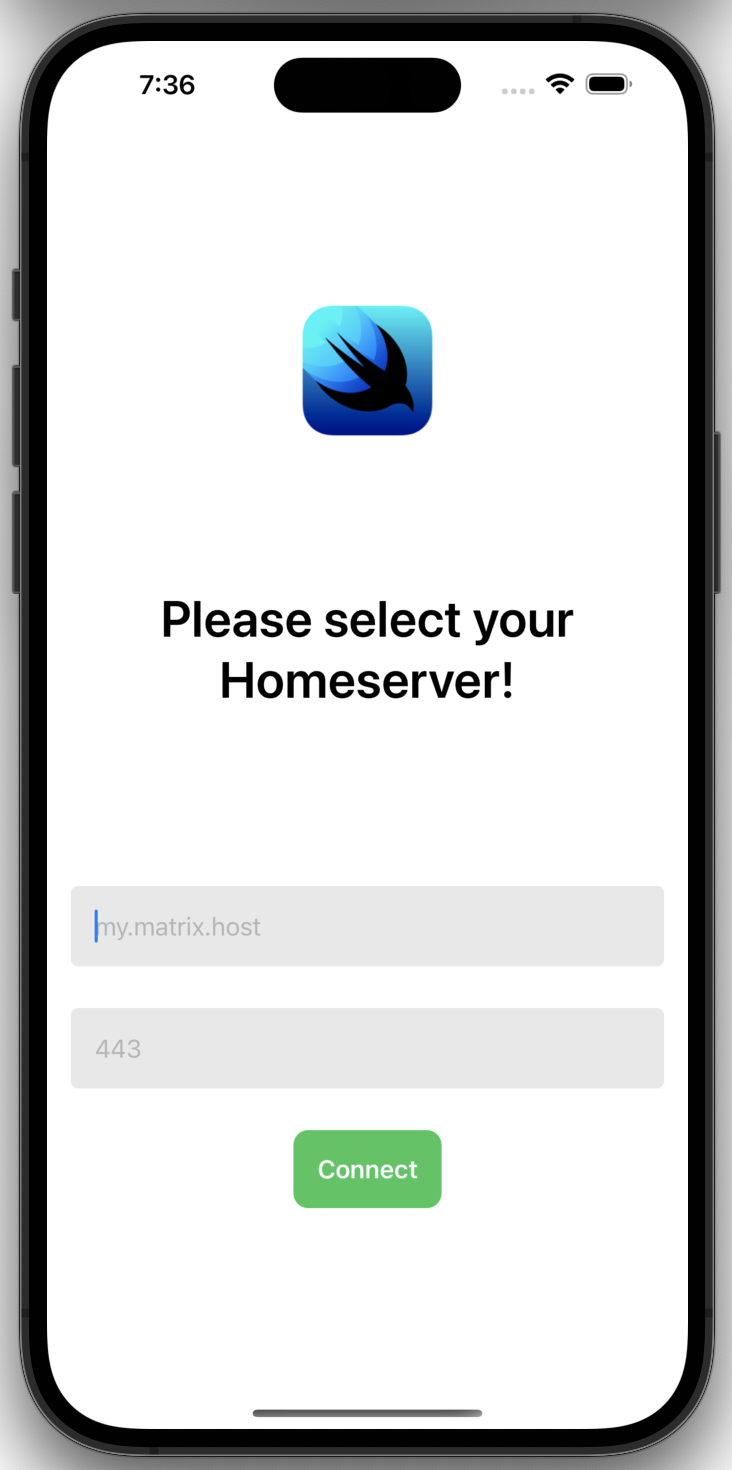
\includegraphics[scale=0.5]{homeserver}
        \centering
        \caption{SelectHomeserverView}\label{fig:selecthomeserverview}
    \end{figure}
%    \begin{wrapfigure}{R}{0.5\textwidth}
%        \begin{center}
%            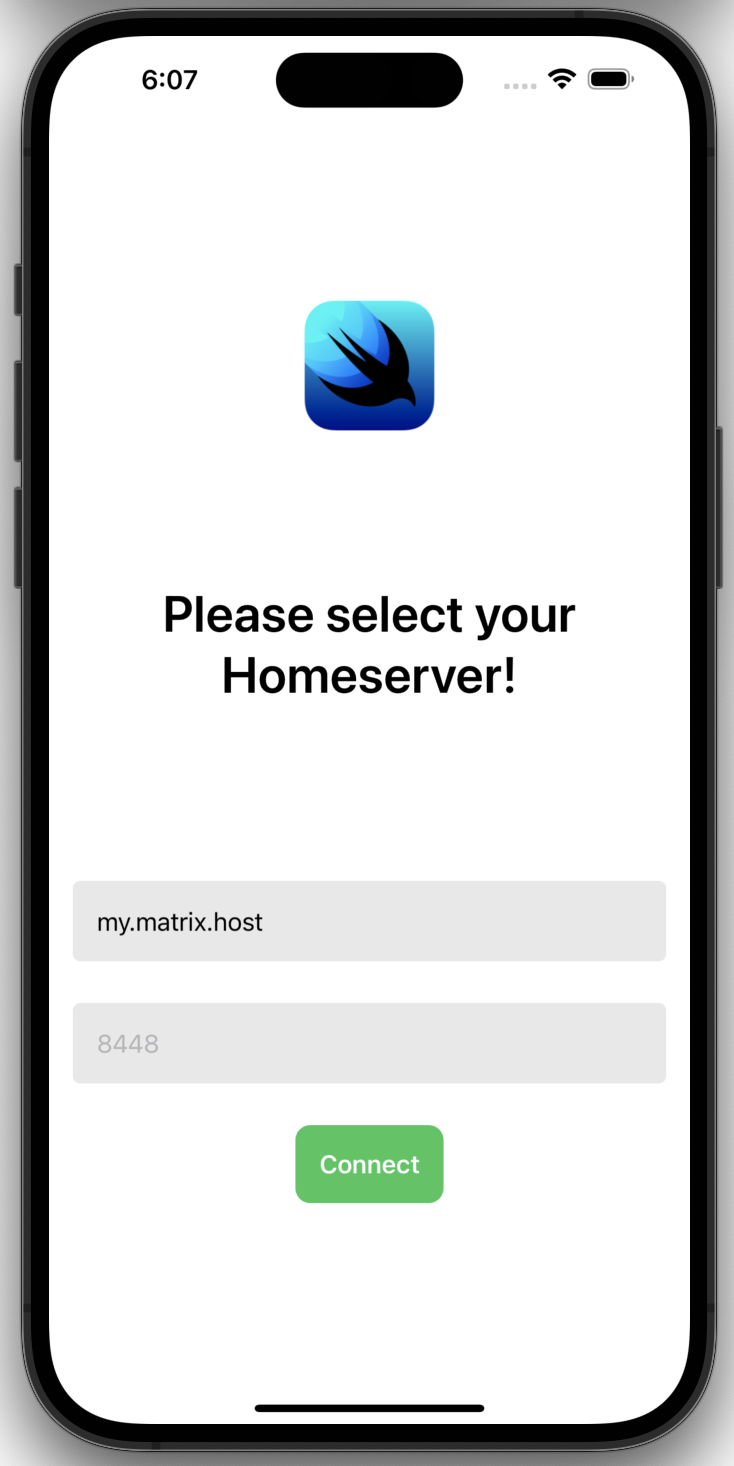
\includegraphics[scale=0.5]{selecthomeserver}
%        \end{center}
%        \caption{SelectHomeserverView}\label{fig:selecthomeserverview}
%    \end{wrapfigure}
    Hat der User einen Homeserver eingetragen und klick auf connect prüft die App zuerst ob der Homeserver erreichbar ist.
    Hierzu wird eine Abfrage der Versionsnummer an den angegebenen Homeserver gesendet.
    Dies geschieht durch senden einer GET Anfrage an \texttt{/\_matrix/client/versions} (siehe Abschnitt~\ref{sec:rest}).
    Ist diese Anfrage erfolgreich wird der Homeserver im Model hinterlegt und der User gelangt zur \texttt{LoginView} welche in Abbildung ~\ref{fig:loginview} zu sehen ist.
    Falls die Anfrage fehlschlägt wird dem User eine Fehlermeldung gezeigt.
    \begin{figure}[h]
        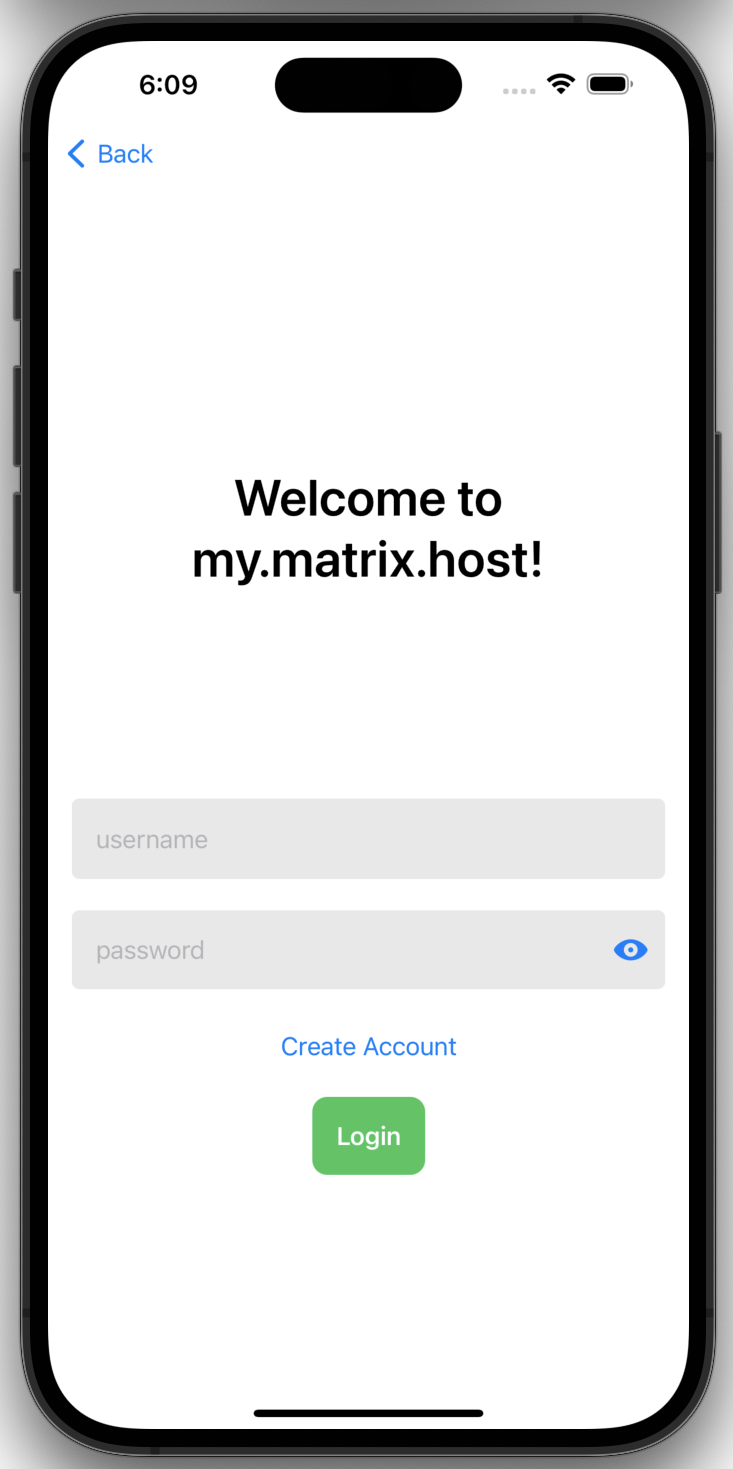
\includegraphics[scale=0.5]{login}
        \centering
        \caption{LoginView}\label{fig:loginview}
    \end{figure}
    In dieser View kann der User sich entweder mit seinem bereits existierenden Account anmelden oder einen neuen Account erstellen.
    Für den Fall, dass der User bereits einen Account besitzt muss er seinen User namen und sein Passwort in die dafür vorgesehenen Felder eintragen und über den Login Button bestätigen.
    Das Passwortfeld ist hierbei ein \texttt{SecureField} welches die Eingabe versteckt und lediglich mit Punkten darstellt.
    Über das Auge am Rand des Textfeldes kann der User zwischen geschützter Ansicht und Klartext wechseln.


    Hat der User seine Zugangsdaten eingegeben und über den Login Button bestätigt wird über den \texttt{MXRestClient}, welcher von der SDK (siehe Abschnitt~\ref{sec:matrix-sdk}) bereit gestellt wird, eine Login-Anfrage mit Usernamen und Passwort an den Server gesendet.
    Bei gültigen zugangsdaten enthält die Antwort des Servers folgende Informationen:
    \begin{description}[leftmargin=!,labelwidth=3cm]
        \item [home\_server] die vollständige Adresse des Homeservers
        \item [access\_token] ein Access Token zur weiteren Verwendung mit dem \texttt{MXRestClient}
        \item [user\_id] die vollständige Matrix ID des Users
        \item [device\_id] die vom Server zugewiesene ID für das Gerät
    \end{description}
    Die Information über \texttt{home\_server}, \texttt{user\_id} und \texttt{device\_id} werden in den \texttt{UserDefaults} der App gespeichert.
    Da der \texttt{access\_token} den Zugriff auf Benutzerkonto des Users ermöglicht, wird dieser mittels eines \texttt{KeychainHelper}\footnote{https://gist.github.com/LeeKahSeng/2452e90a57a5324de367907a36d88a49} in der iCloud Keychain gespeichert.
    Falls die Zugangsdaten nicht korrekt sind wird dem User erneut eine Fehlermeldung gezeigt.
    Anschließend wird mit diesen Information eine Matrix Session gestartet welche vollen Zugriff auf die Nutzerdaten
    War das starten der Session erfolgreich gelangt der User in die \texttt{RoomsView}.\\

    Für Den Fall das der User noch keinen Account besitzt kann über den Button "Create Account" der \texttt{LoginView} zur \texttt{CreateAccountView} gelangen welche in Abbildung~\ref{fig:createaccountview} dargestellt ist.
    Diese View dient der Account erstellung und enthält 3 Textfelder für Benutzernamen, Passwort und Registrierungstoken.
    Für das Passwortfeld kann wie schon in der \texttt{LoginView} zwischen versteckter Eingabe und Klartet gewechselt werden.
    \begin{figure}[h]
        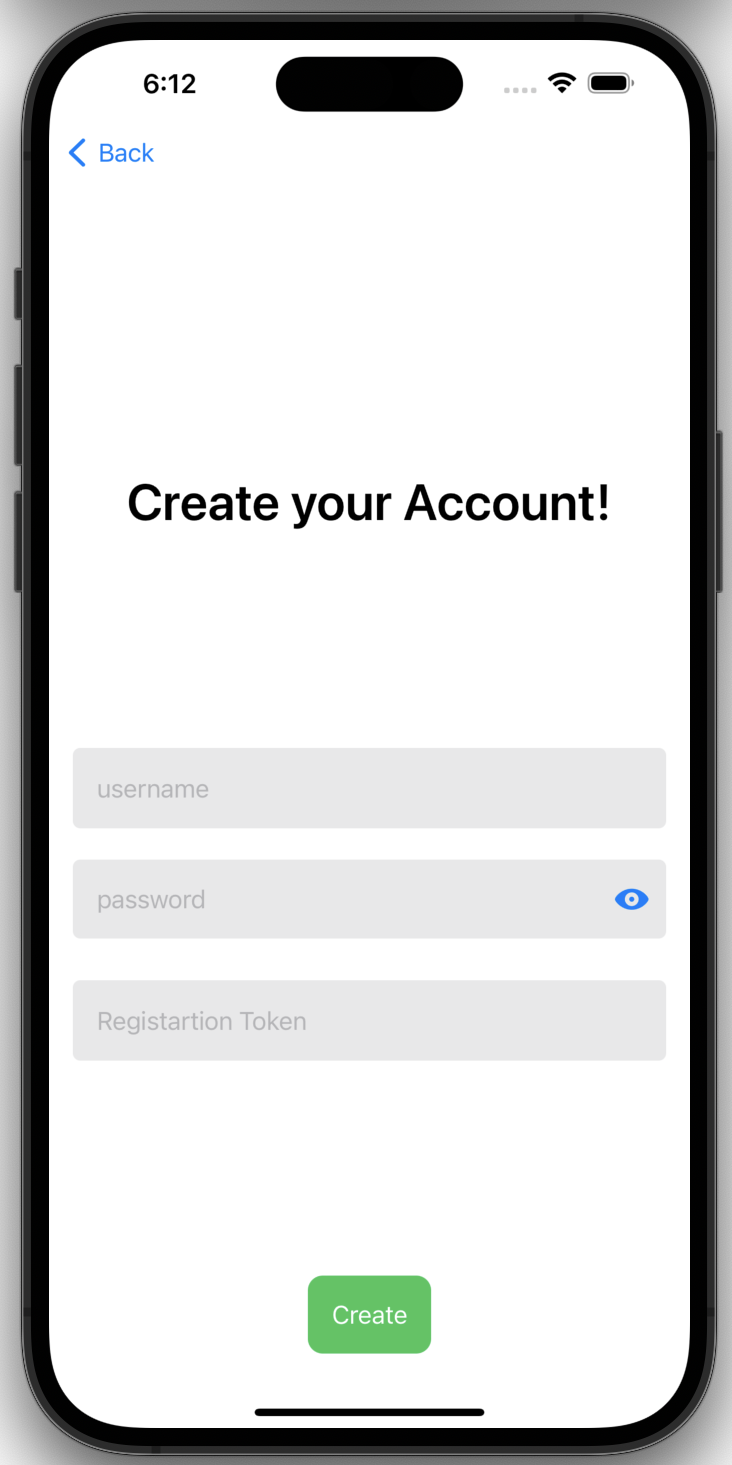
\includegraphics[scale=0.5]{accountcreate}
        \centering
        \caption{CreateAccountView}\label{fig:createaccountview}
    \end{figure}
    Der Registrierungstoken kann über die Admin-API\footnote{https://matrix-org.github.io/synapse/latest/usage/administration/admin\_api/} des Servers erstellt werden.
    Hierzu muss eine GET-Anfrage an \texttt{/\_synapse/admin/v1/registration\_tokens/new} gesendet werden.~\cite{synapseregistartiontoken}
    Alternativ kann auch direkt in der Datenbank des Servers ein Token angelegt werden (im \texttt{registration\_tokens} table).
    Es werden folgende Felder bereitgestellt:
    \begin{description}[leftmargin=!,labelwidth=3cm]
        \item [token] Der Token der bei der Erstellung des Accounts angegeben werden muss.
        \item [uses\_allowed] Die maximale Anzahl an Accounts die mit einem Token erstellt werden kann.
        \item [pending] Anzahl laufender Registrierungen.
        Sie gibt an wie viele Benutzer die Authentifizierungsstufe mit dem Token bereits abgeschlossen haben ohne den vollständigen Registrierungsvorgang erfüllt zu haben.
        \item [completed] Anzahl erfolgreich erstellter Accounts mit diesem Token.
        \item [expiry\_time] Ablaufdatum des Tokens. Er gibt an wie lange der Token gültig ist.
    \end{description}

    Der eigentliche Registrierungsvorgang kann mehrere Authentifizierungsstufen enthalten.
    Bevor der Registrierungsvorgang gestartet wird ir zuvor mit der vom \texttt{MXRestClient} bereitgestellten Funktion geprüft ob der Benutzername bereit genutzt wird.
    In dieser Implementation wird der in Abbildung~\ref{fig:accountCreationDiagram} beschriebene dreistufige Accounterstellungsvorgang mittels eines Registriersungstokes genutzt.

    \begin{figure}[h]
        \centering
        \begin{sequencediagram}
            \newthread{A}{Client}{}
            \newinst[7]{B}{Server}{}
            \begin{sdblock}{Stage 1}{Receive Session ID}
                \begin{call}{A}{getRegistrationSession()}{B}{\shortstack{
                    return Session ID\\
                    return supported flows}}
                    \postlevel
                \end{call}
            \end{sdblock}
            \begin{sdblock}{Stage 2}{m.login.registration\_token}
                \begin{call}{A}{register()}{B}{}
                \end{call}
            \end{sdblock}
            \begin{sdblock}{Stage 3}{m.login.dummy}
                \begin{call}{A}{register()}{B}{}
                \end{call}
            \end{sdblock}
        \end{sequencediagram}
        \caption{Account erzeugungs Flow}
        \label{fig:accountCreationDiagram}
    \end{figure}

    Im ersten Schritt sendet der Client eine leere Anfrage zum Server in welcher er um das starten einer Registrierungssitzung bittet.
    Der Server antwortet daraufhin mit einer SessionID und den vom Homeserver unterstützten Authentifizierungs-Flows.
    In diesem Beispiel ist der einzige unterstützte Flow die verifizierung über einen Registriersungstoken.
    Im nächsten Schritt sendet der Client dann den zuvor bereitgestellten Registrierungstoken und die vom Server gegebene SessionID in Kombination mit der aktuellen Stufe des Authentifizierungsvorgangs.
    Im dritten und letzten Schritt wird nun der dummyflow aufgeführt.
    Dieser Flow kann nicht fehlschlagen und dient der zur finalen Erstellung des Account.
    Hierbei werden der gewünschte Benutzername und Passort übergeben.
    Ist dies geschehen wurde der Account erfolgreich erstellt.
    Anschließend wird der User ebenfalls auf die \texttt{RoomsView} weitergeleitet.

    \newpage
    \subsection{Raumübersicht}\label{subsec:raumubersicht}

    Die \texttt{RoomsView} bildet das Herzstück der App.
    Sie ist die Ansicht die dem User bei jedem Start der App gezeigt wird sofern er sich bereits in der App angemeldet hat.
    Von dieser Ansicht aus können alle weiteren Views erreicht werden.
    Die in Abbildung~\ref{fig:roomsview} gezeigte View besteht aus einer \texttt{Toolbar} im Kopf der Ansicht über welche man zur \texttt{ProfileView} und \texttt{SettingsView} gelangt.
    Darunter findet sich die Raum übersicht welche alle beigetretenen Räume in einer scrollbaren Liste anzeigt.
    Jedes Element der Liste zeigt den das Profilbild des jeweiligen Raumes sowie Displayname oder Title des jeweiligen Raumes.
    Bei direkten Räumen wird außerdem die MatrixID des Users angezeigt.
    Auf der rechten Seite befindet sich der Zeitpunkt der letzten Nachricht und ein Indikator dafür ob und wie viele ungelesene Nachrichten im einem Raum existieren
    Über das darüberliegende Textfeld kann kann die Liste gefiltert werden.
    Darüber hinaus wird die Liste nach dem  \texttt{originServerTimestamp} der letzten Nachricht des jeweiligen Raumes sortiert.

    \begin{figure}[h]
        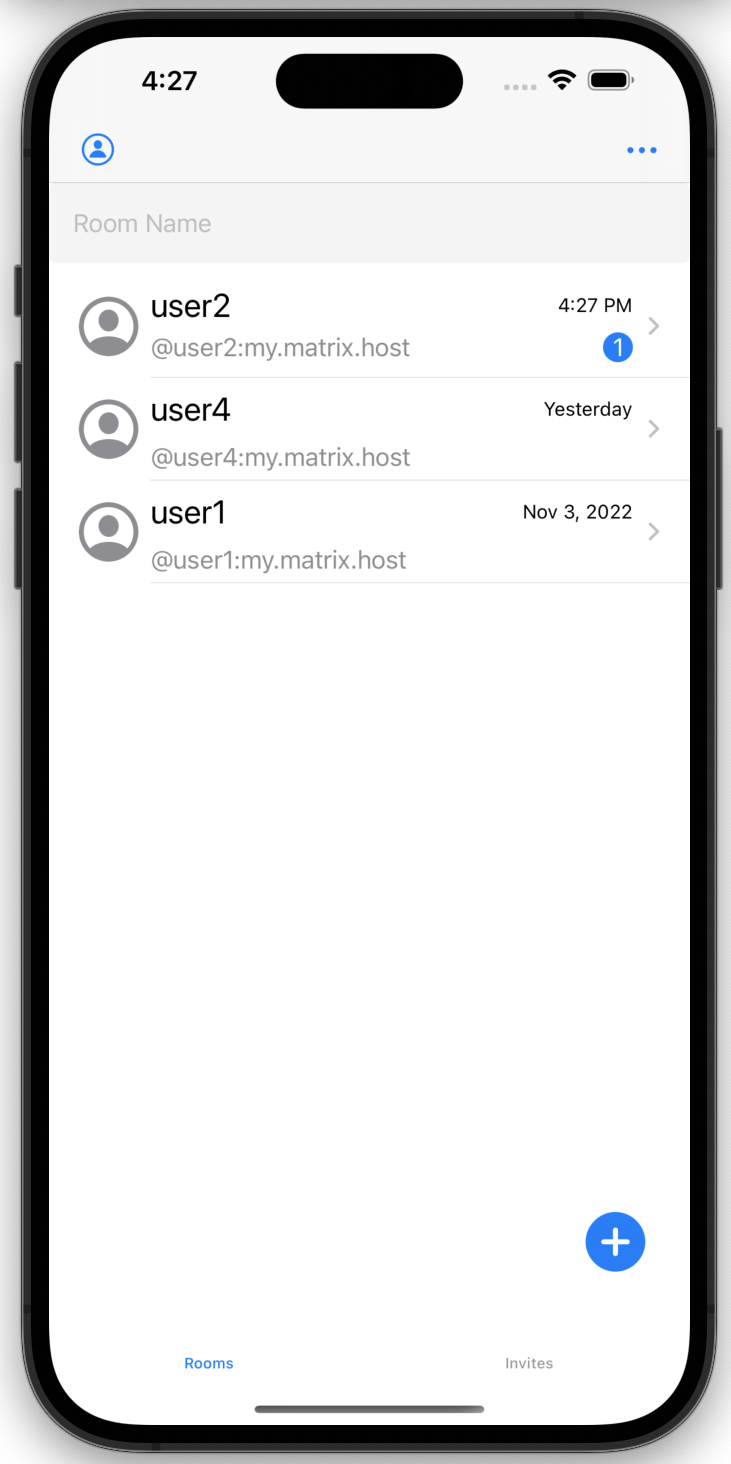
\includegraphics[scale=0.5]{rooms}
        \centering
        \caption{RoomsView}\label{fig:roomsview}
    \end{figure}
    Über den Button mit dem Plus gelangt man zur \texttt{NewRoomView} in welcher man einen neun Raum erstellen kann.
    Im Fuß der View befindet sich eine TabView über welche zwischen \texttt{RoomsView} und \texttt{InvitesView} gewechselt werden kann.
    Die \texttt{InvitesView} welche in Abbildung~\ref{fig:invitesview} zu sehen ist dient dazu alle offenen Einladungen zu anderen Räumen aufzulisten.
    Diesen kann durch einfaches klicken auf den jeweiligen Raum beigetreten werden.
    Man gelangt dann zur \texttt{ChatView} und kann direkt mit dem jeweiligen Raum Kommunizieren.
    Falls man die Einladung ablehnen möchte kann man dies durch wischen der Einladung in Richtung des linken Bildschirmrandes tun.

    \begin{figure}[h]
        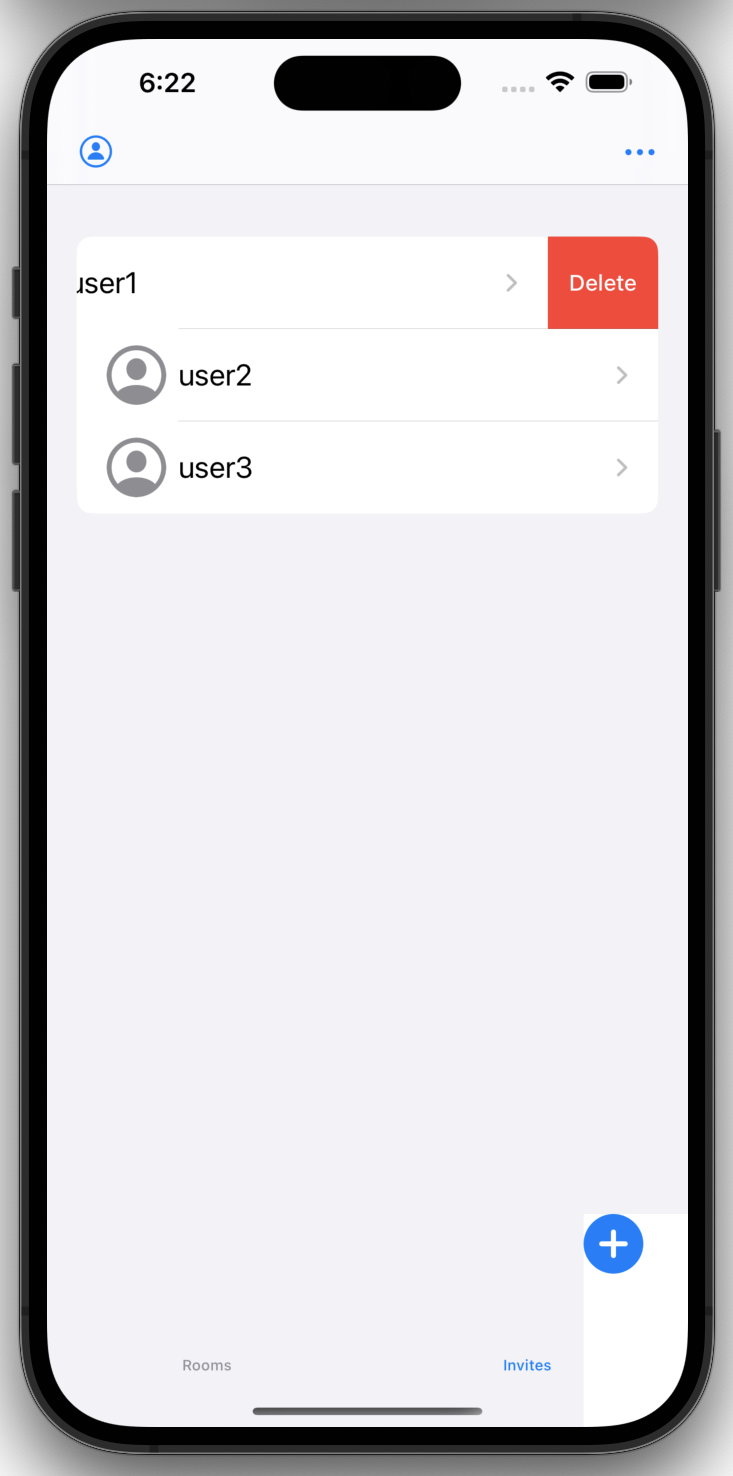
\includegraphics[scale=0.5]{invites}
        \centering
        \caption{InvitesView}\label{fig:invitesview}
    \end{figure}

    \newpage
    \subsection{Raumerzeugung}\label{subsec:raumerzeugung}
    Hat der User in der \texttt{RoomsView} oder \texttt{InvitesView} auf den Plus-Button geklickt gelangt er in die \texttt{NewRoomView}.
    Diese View dient dazu neue Räume zu erstellen und User zu diesen einzuladen.
    Hierzu wird dem User wie in Abbildung~\ref{fig:newroomview} zu sehen, ein Textfeld gezeigt über welches er nach anderen Usern über deren Anzeigenamen oder ihre MatriID suchen kann.
    In der sich in der Unteren hälfte befindlichen scrollbaren Liste werden bis zu 10 Nutzer gezeigt die dem eingegebenen Suchtext entsprechen.
    Diese Funktion ist nur möglich falls in der Konfiguration des Homeservers die suche im Nutzerverzeichnis freigegeben ist.
    Die Konfiguration des Homeservers ist in Abschnitt~\ref{sec:homeserver} genauer beschrieben.
    Ist diese Funktion nicht freigegeben muss der User die vollständige MatrixID des gesuchten Nutzers angeben.
    Hat der User den von ihm gesuchen Nutzer gefunden kann er durch anklicken dem zu erstellenden Raum hinzufügen.
    Der Nutzer erscheint dann in der horizontal scrollbaren Liste von Usern.
    Hat der User einen falschen Nutzer zum Raum hinzugefügt kann er diesen durch antippen des Users in der Liste hinzugefügter Nutzer wieder entfernen.
    Hierbei achtet die App darauf, dass ein Nutzer nicht doppelt hinzugefügt werden kann.

    \begin{figure}[h]
        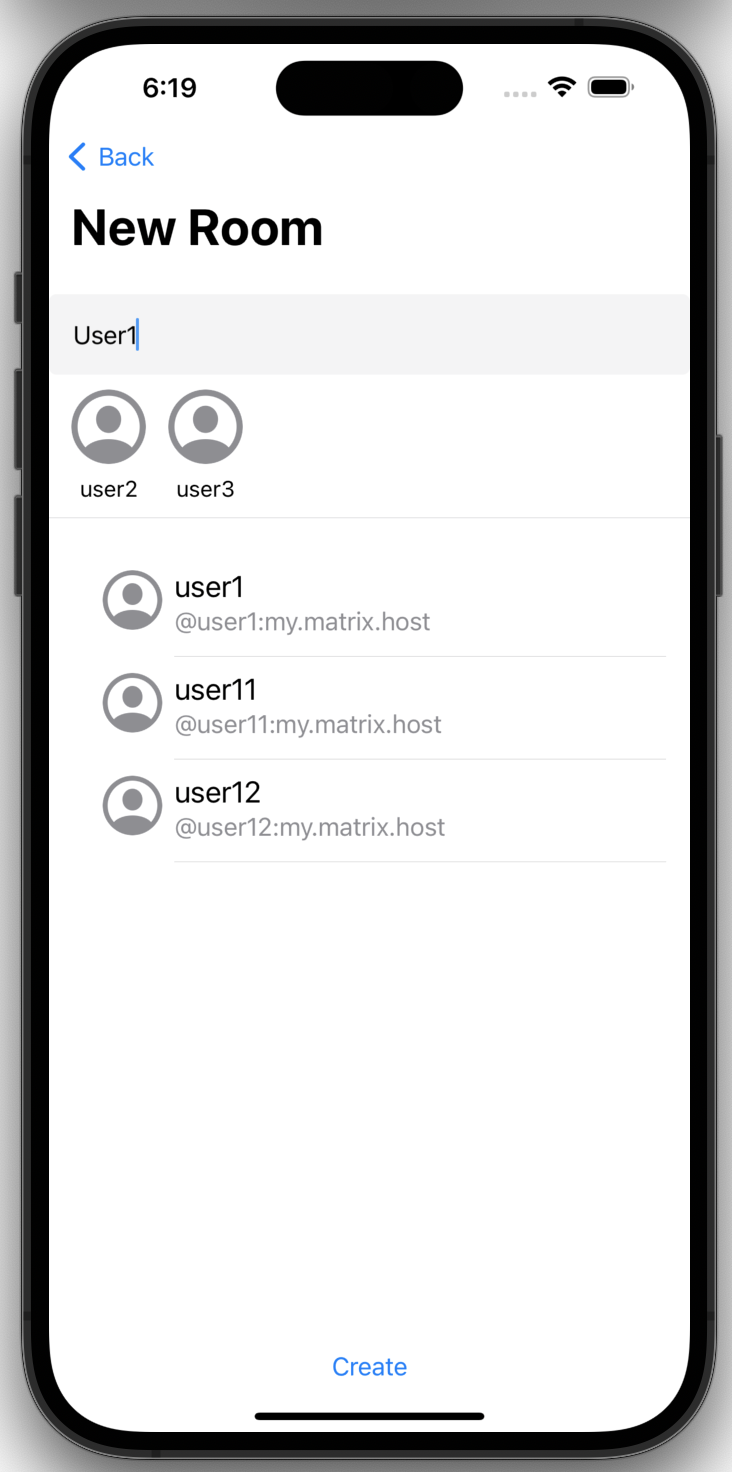
\includegraphics[scale=0.5]{newroom}
        \centering
        \caption{NewRoomView}\label{fig:newroomview}
    \end{figure}

    Hat der User alle von ihm gewünschten Nutzer dem Raum hinzugefügt kann er diesen durch klicken auf den "Create"-Button erstellen.
    Die App entscheidet dann automatisch anhand der Anzahl der eingeladenen Usern ob ein direkter Raum erstellt werden soll oder nicht.
    Nach erstellen der Raumes wird automatisch ein StateEvent von Typ \texttt{.roomEncryption} an den Raum gesendet, welche die anderen Nutzer im Raum darüber informiert das Nachrichten in diesem Raum verschlüsselt zu senden sind.
    Der vollständige Vorgang zum verschlüsseln der Nachrichten ist in Abschnitt~\ref{subsec:verschlusselung-der-nachrichten} beschrieben.
    War das erstellen der Raumes erfolgreich wird der User in die \texttt{ChatView} des neu angelegten Raumes geleitet.

    \newpage
    \subsection{Chatfenster}
    Die in Abbildung~\ref{fig:chatview} gezeigte \texttt{ChatView} ist eine weitere Kernansicht der App.
    Sie ermöglicht es dem User Konversationen eines Raumes einzusehen und neue Nachrichten an diesen zu senden.
    Die Abbildung zeigt Beispielnachrichten für alle unterstützten Nachrichtentypen.
    Es können einfache Textnachrichten versendet werden, Fotos welche durch antippen in einem Fullscreen \texttt{ImageViewer} angezeigt werden,
    PDF-Dateien welche in einem \texttt{PDFViewer} eingesehen werden können, und Videos welche mittels \texttt{AZVideoPlayer} abgespielt werden können.
    Der Videoplayer unterstützt sowohl das abspielen direkt in der \texttt{ChatView} als auch im Fullscreenmode, sowohl im Landscape- als auch im Portrait-format.

    \begin{figure}[h]
        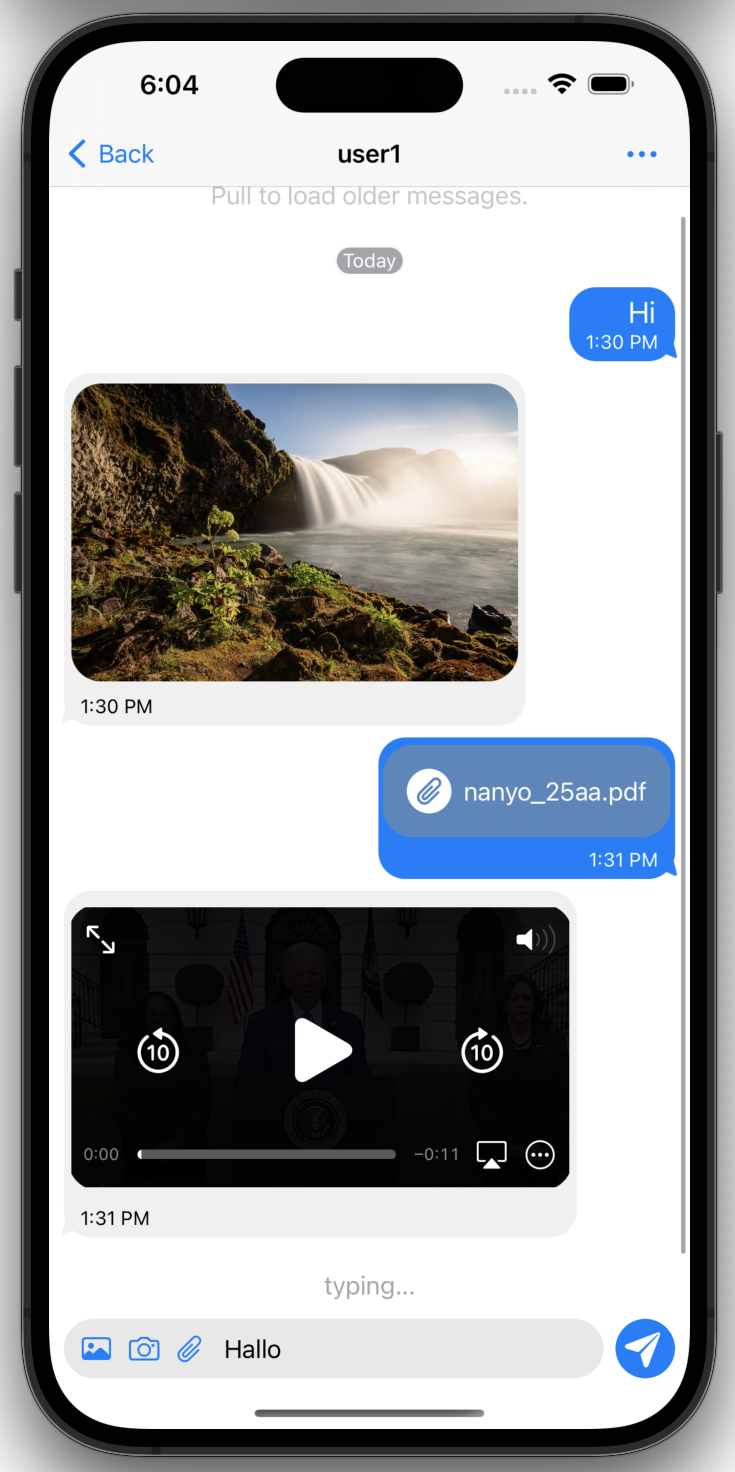
\includegraphics[scale=0.5]{chat}
        \centering
        \caption{ChatView}\label{fig:chatview}
    \end{figure}

    Des weiteren wird dem User ein Typing-Indikator gezeigt welcher der User darüber informiert ob der Gesprächspartner (oder in Multiuser Räumen welche Gesprächspartner) gerade eine Nachricht schreiben.
    Im Fuß der Ansicht befindet sich das Nachrichtenfenster über welches Nachrichten verfasst und an der Raum gesendet werden können.
    Durch klicken des Bild-Icons öffnet sich ein \texttt{ImagePicker} über welchen sowohl Fotos als auch Videos aus der Galerie gewählt und an den Raum gesendet werden können.
    Das Kamera-Icon daneben öffnet eine Kamera Ansicht über welche Fotos und videos direkt aus der App aufgenommen und versendet werden können.
    Über das Büroklammer-Icon lassen sich Dateien die auf dem Gerät gespeichert sind durchsuchen und an den Raum senden.
    Da nur Dateien vom Typ PDF von der App unterstützt werden wird im Datei Picker ebenfalls nach PDF gefiltert.
    Im Kopf der Ansicht erkennt man eine Hinweismeldung darauf, dass man das Ende der geladenen Nachrichten erreicht hat und nach unten wischen muss um weitere Nachrichten zu laden.
    Bei öffnen der \texttt{ChatView} werden sofern vorhanden 25 Nachrichten geladen.
    Dies geschieht mittels pagination der Matrix Timeline eines Raumes.
    Bei jedem weiteren laden von Nachrichten werden 25 weitere Nachrichten geladen und angezeigt.
    Es muss darauf geachtet werden, dass die Reihenfolge der Nachrichten ordnungsgemäß angezeigt wird.
    Die Lazy-Loading-Methode erlaubt hierbei eine angemessene Performance beim öffnen des Chats.
    Eine besondere Herausforderung ist die Position der scrollbaren Liste.
    Beim öffnen der View muss an das Ende der Liste gesprungen werden, da sich dort die neusten Nachrichten befinden.
    Falls eine neue Nachricht eintrifft während die View geöffnet ist springt die Liste ebenfalls an das Ende um dem Nutzer die neuste Nachricht anzuzeigen.
    Beim Laden älterer Nachrichten soll jedoch nicht zum Ende gesprungen werden.
    Über die drei Punkte in der oberen rechten Ecke der Ansicht öffnet sich ein Drop-Down-Menu über welches ein Raum verlassen werden kann oder sich eine Übersicht über den aktuellen Raum öffnet, wo Titel, Beschreibung und Bild des Raumes geändert werden können.
    Darüber hinaus zeigt sie einige Informationen über den Raum an wie die Anzahl an Teilnehmern, den Ersteller des Raumes und ob die Verschlüsselung aktiv ist.

    \newpage
    \subsection{Profile}\label{subsec:profile}
    Die \texttt{ProfileView} welche in Abbildung~\ref{fig:profileview} zu sehen ist erlaubt dem user seinen Account zu verwalten.
    Durch klicken auf das Profilbild öffnet sich der \texttt{ImagePicker}, welcher auch schon in der \texttt{ChatView} genutzt wurde, wodurch der Nutzer ein neues Profilbild setzen kann.
    Außerdem kann er seinen Anzeigenamen ändern.
    Die Matrix ID bleibt hierbei jedoch gleich.
    Darüber hinaus wird dem User die Möglichkeit geboten sein Passwort zu ändern.
    Hierfür öffnet sich nach klicken des Buttons ein alert welcher den Nutzer um Eingabe seines alten und seines neuen Passworts bittet.
    Falls das alte Passwort korrekt eingegeben wurde wird das neue Passwort gesetzt.\\
    Im unteren Teil der Ansicht befinden sich 2 Buttons, ein logout und ein delete Button ..  .. . . .

    \begin{figure}[h]
        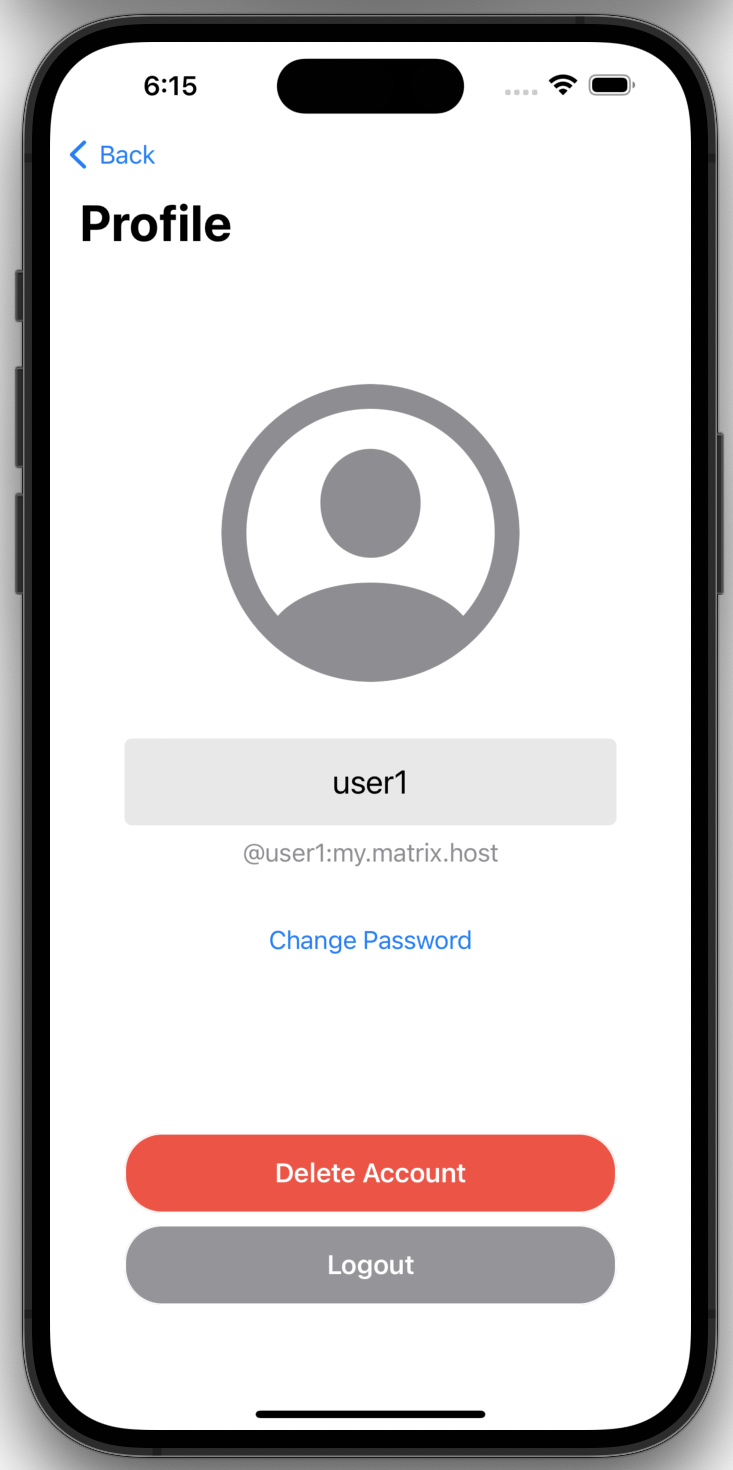
\includegraphics[scale=0.5]{profile}
        \centering
        \caption{ProfileView}\label{fig:profileview}
    \end{figure}

    \begin{figure}[h]
        \centering
        \begin{sequencediagram}
            \newthread{A}{Client}{}
            \newinst[7]{B}{Server}{}
            \begin{sdblock}{Stage 1}{Receive Session ID}
                \begin{call}{A}{getLoginSession()}{B}{\shortstack{
                    return Session ID\\
                    return supported flows}}
                    \postlevel
                \end{call}
            \end{sdblock}
            \begin{sdblock}{Stage 2}{m.login.password}
                \begin{call}{A}{deactivateAccount()}{B}{}
                \end{call}
            \end{sdblock}
        \end{sequencediagram}
        \caption{Account löschen Flow}\label{fig:figure}
    \end{figure}

%    \subsection{Start der Matrix Session}\label{sec:start-der-matrix-session}

    \subsection{Verschlüsselung der Nachrichten}\label{subsec:verschlusselung-der-nachrichten}
    Zur Verschlüsselung der Nachrichten sind mehrere Schritte notending.
    Zuerset muss die Verschlüsselung in der Sitzung aktiviert werden.
    Dies geschieht durch starten und aktivieren des Crypto Modules der SDK.
    Dabei werden die im Abschnitt~\ref{subsec:verwendete-schlussel} aufgeführten Schlüssel erstellt und mit dem Server synchronisiert.
    Zusätzlich mus beim erstellen eines Raumes zuallererst ein encryption Event gesendet werden, welches die anderen Teilnehmer eines Raums darüber informiert, dass die Kommunikation in einem Raum verschlüsselt zu erfolgen hat.
    Hierbei muss der für die Verschlüssleung der Nachricht verwendete Algorithmus angegeben werden.
    Zur Zeit wird nur die \texttt{m.megolm.v1.aes-sha2} Verschlüsselung von der SDK unterstützt.
    Falls nun eine Nachricht über die Sitzung an den erstellten Raum gesendet wird, wird diese beim senden automatisch von der SDK verschlüsselt.
    Beim Empfangen von Nachrichten wird das Event ebenfalls automatisch entschlüsselt.
    Bei Fotos, Videos und Datein ist zu beachten, dass das Event lediglich einen Pfad zum Ablageort der gesendeten Datei auf dem Server enthält.
    Dieser Pfad muss nun übersetzt werden und anschließend heruntergeladen werden.
    Da die Dateien nach dem herunterladen noch immer verschlüsselt sind müssen diese anschließend mit der von der SDK bereitgestellten Funktion \texttt{MXEncryptedAttachments.decryptAttachment()} separat entschlüsselt werden.
    Anhand der Notwendigkeit des entschlüsselns der Dateien kann bestätigt werden, dass die Verschlüsslung aktiv ist.
    Zusätzlich kann auf dem Homeserver unter \texttt{/data/media\_store} geprüfte werden, dass die Dateien verschlüsselt auf dem Server abgelegt werden.

    \subsection{Benachrichtigungen}\label{subsec:benachrichtigungen}


    \newpage
    \section{Homeserver}\label{sec:homeserver}
    Der Homeserver bildet die unterliegende Infrastruktur der Plattform.
    Hierfür wird das vom Matrix Team bereitgestellte Synapse Docker Image verwendet.
    Diese wird in einem Docker Container auf dem Server betrieben.
    Bevor der Container gestartet werden kann, werden einige Konfigurationsdateien benötigt welche über folgenden Befehl generiert werden können:
    \begin{lstlisting}[language=bash,label={lst:synapse-generate}]
docker run -it --rm -v /path/on/host/machine/:/data -e SYNAPSE_SERVER_NAME=my.matrix.host -e SYNAPSE_REPORT_STATS=yes matrixdotorg/synapse:latest generate
    \end{lstlisting}
    Um später einfacher Änderungen an der Konfiguration des Homeservers vornehmen zu können wird das \texttt{/data} Directory im Host gemounted.
    Des weiteren muss der Name des Homeservers über \texttt{SYNAPSE\_SERVER\_NAME} definiert werden.
    Dieser wird später für die Identifikation des Homeservers genutzt.
    Nach ausführen des Befehls werden 3 Dateien generiert:
    \begin{description}[leftmargin=!,labelwidth=4cm]
        \item [homeserver.yaml] Konfigurationsdatei des Homeservers. Hier können alle Funktionalitätet des Homeservers konfiguriert werden.
        \item [my.matrix.host.log.config] Konfigurationsdatei des Loggers. Hier kann das Fromat für Log-Messages definiert werden und weitere
        \item [my.matrix.host.signing.key] Key zur Authentifizierung bei anderen Homeservern
    \end{description}

    Der \texttt{my.matrix.host.signing.key} wird für diese Implementation nicht benötigt, da der einzeln läuft und nicht an das Matrix Netzwerk angeschlossen wird.
    Bevor der Server gestartet wird sollten noch einige Konfigurationen angepasst werden:
    \begin{enumerate}[label={(\arabic*)}]
        \item Standardmäßig wird nur ein Listener auf Port 8008 für ungeschützte Verbindungen über HTTP konfiguriert.
                Um die App mit dem Homeserver verbinden zu können muss ein zusätzlicher HTTPS Listener auf Port 443 konfiguriert werden.
            \begin{lstlisting}[language=yaml,label={lst:listener}]
listeners:
  - port: 443
    type: http
    tls: true
    resources:
          - names: [client, federation]
            \end{lstlisting}
        \item Für den zusätzlichen Listener über HTTPS muss ein SSL Zertifikat erstellt werden und in der Konfiguration hinterlegt werden. Während der Entwicklung wurde hierfür ein selbst signiertes Zertifikat mittels Open SSL generiert.
            \begin{lstlisting}[language=yaml,label={lst:ssl-certificate}]
tls_certificate_path: "/data/certs/cert.pem"
tls_private_key_path: "data/certs/key.pem"
            \end{lstlisting}
        \item Da der Server nicht mit dem Matrix Netzwerk verbunden wird muss die Key Verifizierung über den Matrix Root Server deaktiviert werden.
            \begin{lstlisting}[language=yaml,label={lst:disable-key-verification}]
federation_verify_certificates: false
trusted_key_servers:
  - server_name: "matrix.org"
    accept_keys_insecurely: true
    enable_registration_without_verification: true
            \end{lstlisting}
        \item Um das in Abschnitt~\ref{subsec:raumerzeugung} beschriebene durchsuchen des Nutzerverzeichnisses zu ermöglichen muss dies hier erlaubt werden.
            \begin{lstlisting}[language=yaml,label={lst:user-directory}]
user_directory:
  enabled: true
  search_all_users: true
            \end{lstlisting}
        \item Zusätzlich können Regeln aktiviert werden die beim Erstellen eines Account Prüfen ob das Passwort den gewünschten Richtlinien entspricht.
                Hier kann definiert werden welche Arten von Zeichen im Passwort enthalten sein müssen und wie lang das Passwort mindestens sein muss.
            \begin{lstlisting}[language=yaml,label={lst:password-policy}]
password_config:
   enabled: true
   localdb_enabled: true
   pepper: "EVEN_MORE_SECRET"

   policy:
      enabled: true
      minimum_length: 8
      require_digit: true
      require_symbol: true
      require_lowercase: true
      require_uppercase: true
            \end{lstlisting}
        \item Da die Registrierung nur mit einem Registrierungstoken möglich sein soll muss dies ebenfalls angegeben werden.
        \begin{lstlisting}[language=yaml,label={lst:enable-registration}]
enable_registration: true
registration_requires_token: true
        \end{lstlisting}
    \end{enumerate}

    Nachdem alle Konfigurationen getätigt wurden kann der Homeserver gestartet werden.
    Es ist darauf zu achten, dass alle benötigten Ports des Containers auf dem Host gemapped werden.

    \begin{lstlisting}[language=bash,label={lst:synapse-start}]
docker run -d --name synapse -v /path/on/host/machine/:/data -p 8008:8008 -p 443:443 matrixdotorg/synapse:latest
    \end{lstlisting}

    Nach dem Start des Containers ist der Homeserver einsatzbereit und Clients können eine Verbindung aufnehmen.

    \newpage
    \chapter{Evaluation}\label{ch:evaluation}
    In diesem Kapitel werden die in Abschnitt~\ref{sec:anforderungen} definierten Anforderungen auf ihre Implementation geprüft.
    Hierbei werden die mit Won't priorisierten Anforderungen nicht beachtet.

    \newpage
    \section{Must-Anforderungen}\label{sec:must-anforderungen}
    \begin{table}[h]
        \centering
        \begin{tabular}{p{0.47\textwidth}|p{0.47\textwidth}}
            Anforderung & Status\\
            \cline{1-2}
            Der User muss über die App einen Account auf der Plattform anlegen können.
            &  \textbf{Erfüllt} \\
            \cline{1-2}
            Der User muss sich mit seinem Account in der App einloggen können. &  \textbf{Erfüllt} \\
            \cline{1-2}
            Der User muss sein Passwort ändern können. & \textbf{Erfüllt}  \\
            \cline{1-2}
            Dem User muss alle von beigetretenen Räume sehen können. &  \textbf{Erfüllt} \\
            \cline{1-2}
            Dem User muss neue Räume erstellen können. & \textbf{Erfüllt} \\
            \cline{1-2}
            Der User muss zu neuen Räumen eingeladen werden können. & \textbf{Erfüllt} \\
            \cline{1-2}
            Der User muss alle Nachrichten die in einem Raum gesendet wurden einsehen können. & \textbf{Erfüllt} \\
            \cline{1-2}
            Der User muss Nachrichten in einem Raum senden können. & \textbf{Erfüllt} \\
            \cline{1-2}
            Nachrichten zwischen Usern müssen End-to-End Verschlüsselt sein. & \textbf{Erfüllt} \\
            \cline{1-2}
            Der User muss einen Raum verlassen können. & \textbf{Erfüllt} \\
            \cline{1-2}
            Der User muss seinen Account deaktivieren können. & \textbf{Erfüllt} (kein automatisches Löschen der Daten erfolgt)\\
            \cline{1-2}
            Die App darf keinen Zugriff auf das Adressbuch des Endgerätes haben. & \textbf{Erfüllt}
        \end{tabular}
        \caption{Übersicht über erfüllte Must-Anforderungen}
        \label{tab:erfüllte-must-anforderungen}
    \end{table}

    \newpage
    \section{Should-Anforderungen}\label{sec:should-anforderungen}
    \begin{table}[h]
        \centering
        \begin{tabular}{p{0.47\textwidth}|p{0.47\textwidth}}
            Anforderung & Status\\
            \cline{1-2}
            Beim erstellen des Accounts soll eine zusätzliche Authentifizierungsmethode verwendet werden um Wahloses erstellen zon Accounts zu verhindern.
            &  \textbf{Erfüllt} (mittels Registrierungstoken)\\
            \cline{1-2}
            Der User soll sich nur einmal einloggen müssen. &  \textbf{Erfüllt} \\
            \cline{1-2}
            Der User soll sich ausloggen können. & \textbf{Erfüllt}  \\
            \cline{1-2}
            Der Benutzer soll die Möglichkeit haben sein Profilbild und seinen Anzeigenamen anzupassen. &  \textbf{Erfüllt} \\
            \cline{1-2}
            Der vollständige Chat-Verlauf soll nur bei Bedarf geladen werden. & \textbf{Erfüllt} (Lazy-Loading)\\
            \cline{1-2}
            Die App soll neben Textnachrichten auch andere Nachrichtentypen wie Fotos, Videos oder Audiodateien unterstützen. & \textbf{Teilweise erfüllt} (unterstützt Foto, Video und PDF) \\
            \cline{1-2}
            Die App soll den User über den Erhalt einer neuen Nachricht informieren. & \textbf{Erfüllt} \\
            \cline{1-2}
            Der User muss Nachrichten in einem Raum senden können. & \textbf{Erfüllt} \\
            \cline{1-2}
            Die Übersicht der beigetretenen Räume soll nach letzter Aktivität sortiert werden. & \textbf{Erfüllt}
        \end{tabular}
        \caption{Übersicht über erfüllte Should-Anforderungen}
        \label{tab:erfüllte-should-anforderungen}
    \end{table}

    \newpage
    \section{Could-Anforderungen}\label{sec:could-anforderungen}
    \begin{table}[h]
        \centering
        \begin{tabular}{p{0.47\textwidth}|p{0.47\textwidth}}
            Anforderung & Status\\
            \cline{1-2}
            Die Liste der beigetretenen Räume kann gefiltert werden. &  \textbf{Erfüllt} \\
            \cline{1-2}
            Dem Erstellen eines Raumes kann dem User eine Liste von Usern vorgeschlagen werden, welche dem gesuchten Namen entsprechen. & \textbf{Erfüllt}  \\
            \cline{1-2}
            Dem User kann ein Typing-Indikator gezeigt werden. &  \textbf{Erfüllt} \\
            \cline{1-2}
            Die App kann auch mit anderen Homeservern verbunden werden. & \textbf{Teilweise erfüllt} (Accounterstellung nicht möglich)\\
            \cline{1-2}
            Der User kann den Inhalt einer Textnachricht in die Zwischenablage kopieren. & \textbf{Nicht erfüllt} \\
            \cline{1-2}
            Der User kann eine Nachricht weiterleiten. & \textbf{Nicht erfüllt}  \\
            \cline{1-2}
            Der User kann eine Nachricht löschen. & \textbf{Nicht erfüllt}  \\
            \cline{1-2}
            Der User kann Dateien welche in einem Raum verschickt wurden herunterladen. & \textbf{Nicht erfüllt}  \\
            \cline{1-2}
            Die App kann im Landscape mode genutzt werden. & \textbf{Teilweise erfüllt}
        \end{tabular}
        \caption{Übersicht über erfüllte Could-Anforderungen}
        \label{tab:erfüllte-could-anforderungen}
    \end{table}


    \chapter{Fazit}\label{ch:fazit}
    Die Plattform erfüllt die grundlegenden Anforderungen welche man an eine Messanger-App hat.
    Sie bietet die Möglichkeit einen Account anzulegen, zu verwalten und wieder zu löschen.
    Sie erlaubt das erstellen, beitreten und löschen von Räumen sowohl in 1-zu-1 als auch in Gruppenräumen.
    Das senden und empfangen von Nachrichten geschieht in echtzeit und mit End-to-End Verschlüsselung, sodass der betreiber der Platform keinerlei Zugriff auf die Daten der Nutzer hat.
    Dabei unterstützt die Platform die gängigsten Nachrichtentypen und informiert den Nutzer über das eintreffen neuer Nachrichten.\\
    Betrachtet man jedoch die Anforderungen welche von der DSGVO an eine Messaging-App im medizinischen Bereich gestellt werden muss man feststellen, dass eine vielzahl weiterer Funktionen implementiert werden müssen bevor sie als DSGVO konform eingestuft werden kann und somit zum Einsatz in der Praxis zugelassen wird.
    Das Matrix Protokol unterstützt den Großteil der notwendigen Implementierungen um DSGVO konform zu werden.
    Die einzige nicht unterstützte Funktionalität die während der Implementation entdeckt wurde ist das Löschen von Nachrichten bzw. Inhalten auf dem Server.
    Hierzu wird vom Protokol zur Zeit noch keine Möglichkeit bereitgestellt und somit muss ein eigenes System zum löschen der Daten entwickelt werden.
    Es ist jedoch möglich über ein \texttt{m.room.redaction} Event den Inhalt einer Nachricht unkenntlich zu machen.\\
    Zwar sind alle Nachrichten und Daten die in einem Raum versendet wurden Verschlüsselt und vor unbefugtem Zugriff geschützt, allerdings ist es dem Betreiber der Plattform möglich die Mitgliedschaften von Nutzern zu Räumen einzusehen.
    Somit könnte abgeleitet werden, welche Personen welche Ärzte besuchen.
    Ob dies zulässig ist müsste separat untersucht werden.

%    Zwar wurde während der Implementierung darauf geachtet, dass jegliche Daten zwischen Arzt und Patient verschlüsselt und vor unbefugtem Zugriff geschützt sind, jedoch müsste die genaue Rechtslage zum Einsatz der Plattform genauer untersucht werden.
%    Das Userinterface der App erfüllt zwar die gesetzten Ansprüche jedoch lässt das Design noch deutlich Platz für Verbesserungen.
%    Alle im Kapitel~\ref{sec:anforderungen} als 'Must' definierten Funktionen sind implementiert.
%    Ebenfalls wurden alle Anforderungen aus der

    \chapter{Ausblick}\label{ch:ausblick}
    Der nächste Schritt in der Entwicklung der Plattform sollte es sein die Cross-Signing-Funktion der End-to-End Verschlüsslung zu unterstützen.
    Hierzu muss ein geeignetes Key-Management-System implementiert werden welches es ermöglicht ein Gerät von einem anderen zu verifizieren und die Private Keys die zur Verschlüsselung der Nachrichten verwendet wurden zwischen den Geräten zu synchronisieren.
    Darüber hinaus sollte eine Prozess implementiert werden der es ermöglicht auch ohne Zugriff auf eines der anderen Geräte die verwendeten Schlüssel wiederherzustellen.
    Somit könnte beispielsweise bei Verlust oder bei Beschädigung des Gerätes trotzdem noch auf bestehende Chat-Verläufe zugegriffen werden.
    Mittels des Recovery Services des Crypto Moduls kann ein Backup der Session Keys auf der Server angelegt werden, welches über einen Recovery Key oder eine Passphrase geschützt werden kann.
    Von diesem Backup können dann bei Bedarf alle gespeicherten Keys wiederhergestellt werden.
    Die Dokumentation hierfür ist noch in der Erstellung~\cite{advancede2e} was die Implementation zum aktuellen Zeitpunkt deutlich erschwert.\\
    Des weiteren kann die Plattform um zusätzliche Nachrichtentypen erweitert werden.
    Es könnte beispielsweise das Aufnehmen und versenden von Audiodateien hinzugefügt werden.
    Außerdem kann der Datei-Message-Typ um weiter Dateitypen erweitert werden.

%    Außerdem könnte ein zusätzlicher Layer implementiert werden, welcher es ermöglicht Informationen über beigetretene Räume und deren jeweilige Konversationen geschützt auf dem Gerät zu speichern.
%    Somit hat der User auch ohne bestehende Verbindung zum Internet, Zugriff auf seine Konversationen und mögliche geteilter Daten.
%    Ferner sollten zusätzliche Dateitypen für Nachrichten unterstützt werden um es
%
%    Des weiteren könnte untersucht werden ob der Synapse Server in der LAge ist den Registrierungstoken über einen SMTP Server direkt an den User zu schicken nach vorheriger angabe einer emailadresse.

%\include{source/content/Test}

%Das Fazit
%\include{source/content/Fazit}
%Einbinden des Abbildungsverzeichnisses

    \backmatter
%Liste der Tabellen
    \listoftables
%Einbinden des Tabellenverzeichnisses
    \listoffigures
%Einbinden des Sourcecodeverzeichnisses
%\lstlistoflistings

% Quellenverzeichnis
    \bibliographystyle{abbrvnat}
    \bibliography{Bachelorarbeit}

% Anhang
    \appendix

\end{document}



%
% EOF
%